%\section{Delta-kick dynamics}
\section{Introduction}

The use of delta-kicked Hamiltonians are common in the study of chaotic systems \cite{CT:Ullah_epjd_2012,CT:White_njp_2014}. The delta-kicked rotor is a prime example of such a system that exhibits chaotic motion following a series of successive kicks. Another such model, building upon the kicked rotor, is the kicked harmonic oscillator, wherein the Hamiltonian acquires an additional quadratic potential. The behaviour of such systems have been well studied \cite{CT:Berman_nonlin_1991, CT:Duffy_pra_2004}, and are interesting models to examine the onset of chaos in both classical and quantum mechanical systems. By converting the conjugate variables to quantum operators, the quantum mechanical analogues can be examined. Granted, chaos in the quantum mechanical world differs from that of the classical world (e.g. quantum unitary evolution), insights may be gained from the study of systems on the boundary between the quantum and classical world.

Here I propose such a system, given a rapidly Bose-Einstein condensate featuring a well ordered vortex lattice. The goal is to generate chaotic motion of the vortices in the condensate through kicking with an optical lattice having a period given by the rotation and translational symmetry of the vortex lattice. Since it is known that the vortex lattice is an Abrikosov lattice with 6-fold symmetry, one can say that given a rotation frequency of $\Omega$, the lattice will return to the same orientation after a rotation of $\Omega/6$. Thus, I can kick the system at this interval with a stationary optical lattice potential, without the need to rotate with the system, making this more experimentally realistic. While the expected dynamics of vortices were not observed in the proposed system, additional interesting behaviour was seen. Thus, I will continue to discuss the model of the system, and the observed dynamical behaviour will be described.

\section{Model}
For the purpose of this work the standard single component Bose--Einstein condensate in a radially symmetric trap of frequency $\omega_\perp$ was assumed. By tightly confining the condensate along the $z$-dimension, with trapping frequency $\omega_z$, such that $\omega_z >> \omega_\perp$, the condensate enters a pancake-shaped geometry. Since the energy required to excite any higher modes along $z$ is $\geq \hbar\omega_z$, one can assume all excitations are planar along the radial coordinate $x-y$ axes, with the $z$ axis in the harmonic oscillator ground state. Modelling of this system is performed in the mean-field limit, given by the Gross--Pitaevskii equation, with Hamiltonian

\begin{equation}\label{eqn:gpe_h0}
	H_{\mathrm{GP}} = -\frac{\hbar^2}{2m}\nabla^2 + \frac{1}{2}m\omega_{\perp}^2\mathbf{r}^2 + g\vert\Psi(\mathbf{r},t)\vert^2.
\end{equation}

Here $g$ describes the interaction between atoms in the condensate, given by \begin{equation}
g = \frac{4\pi\hbar^2a_s}{m},
\end{equation}
where $a_s$ is the s-wave scattering length of the atomic species. Restricting the system to a two-dimensional geometry also requires the move to an effective interaction which encompasses the net effect of the $z$-dimension. This is enabled by scaling the interaction by the length of the harmonic oscillator along the $z$-dimension, and becomes
\begin{equation}
g_{2D} = g\sqrt{\frac{m\omega_\perp}{2\pi\hbar}}.
\end{equation}

To generate vortices in the condensate angular momentum must be added to the system. Experimentally, this can be achieved by various techniques, such as stirring the condensate with a blue-detuned beam \cite{Vtx:Raman_prl_2001}, by carefully inverting the trap bias field potential \cite{Vtx:Kawaguchi_pra_2004}, or through use of artificial gauge fields \cite{AO:Dalibard_rmp_2011}, to name but a few. Numerically, this is achieved by assuming that the system is in the co-rotating frame with the condensate, and accounted for by addition of an angular momentum operator along to the Hamiltonian scaled by rotation frequency, $\Omega L$. The time dependent dynamics of the system can be analysed using the form
\begin{equation}\label{eqn:gpe2d}
	i\hbar\frac{\partial}{\partial t}\Psi(\mathbf{r},t) = \left[ H_{\text{GP}}  -  \Omega_z L_z \right] \Psi(\mathbf{r},t),
\end{equation}
where $\Omega_z$ is the angular frequency and $L_z = xp_y - yp_x$ is the angular momentum operator both about the $z$-axis. This is the form of \ref{eqn:gpe} for a two-dimensional harmonically trapped condensate. If the angular rotation frequency approaches the condensate trapping frequency, $\Omega_z \approx \omega_\perp$ the condensate gains a large triangular lattice of vortices. Assuming an upper limit frequency of $\Omega = 0.995\omega_\perp$ allows the system to have a very large vortex lattice, and still be described capably by mean-field theory. Further increases in the rotation frequency would allow the condensate to enter into a strongly correlated regime, and will no longer be described using Gross--Pitaveskii theory.

As I am interested in lattice ordering effects, the assumption that the trapping frequency along the $z$-axis, $\omega_z$, being much larger than the one along the transverse axis, $\omega_\perp$, allowing the condensate to enter a pancake-shaped geometry is valid~\cite{BEC:Fetter_revmodphys_2009}. Neglecting the $z$ dimension ($\textbf{r}\equiv [x,y]$) simplifies the analysis of the system and resulting dynamics. For this work eq.~\eqref{eqn:gpe2d} will be numerically solved, using the pseudospectral Fourier split operator method making use of GPU computing\cite{NUMERICS}. For realistic experimental parameters I assumed  $N=4.9\times 10^5$ atoms of $^{87}$Rb, with an s-wave scattering length of $a_s=4.76\times10^{-9}$ m~\cite{AO:Roberts_prl_1998}.

The numerically evaluated ground-state for the given set of parameters is shown in Fig.~\ref{fig:vlatt_gnd}, and it can be characterised by the filling factor (or filling fraction) $\nu=N/N_v$, i.e.~the ratio of atoms to vortices discussed in Sec.~\ref{sec:intro}. Values of $10 \leq \nu \leq 1000$ enter the so-called ``mean-field quantum Hall'' regime, with Gross--Pitaevskii theory working well. For values $\nu \leq 10$ the system is said to be strongly correlated. For the chosen parameters, the number of vortices within the visible density region is approximately 600, giving a filling factor of $\nu \approx 800 $. This places the system within the mean-field quantum Hall regime, and therefore a description using Gross--Pitaevskii theory is adequate~\cite{Vtx:Schweikhard_prl_2004}

\begin{figure}[tb]
    \centering
    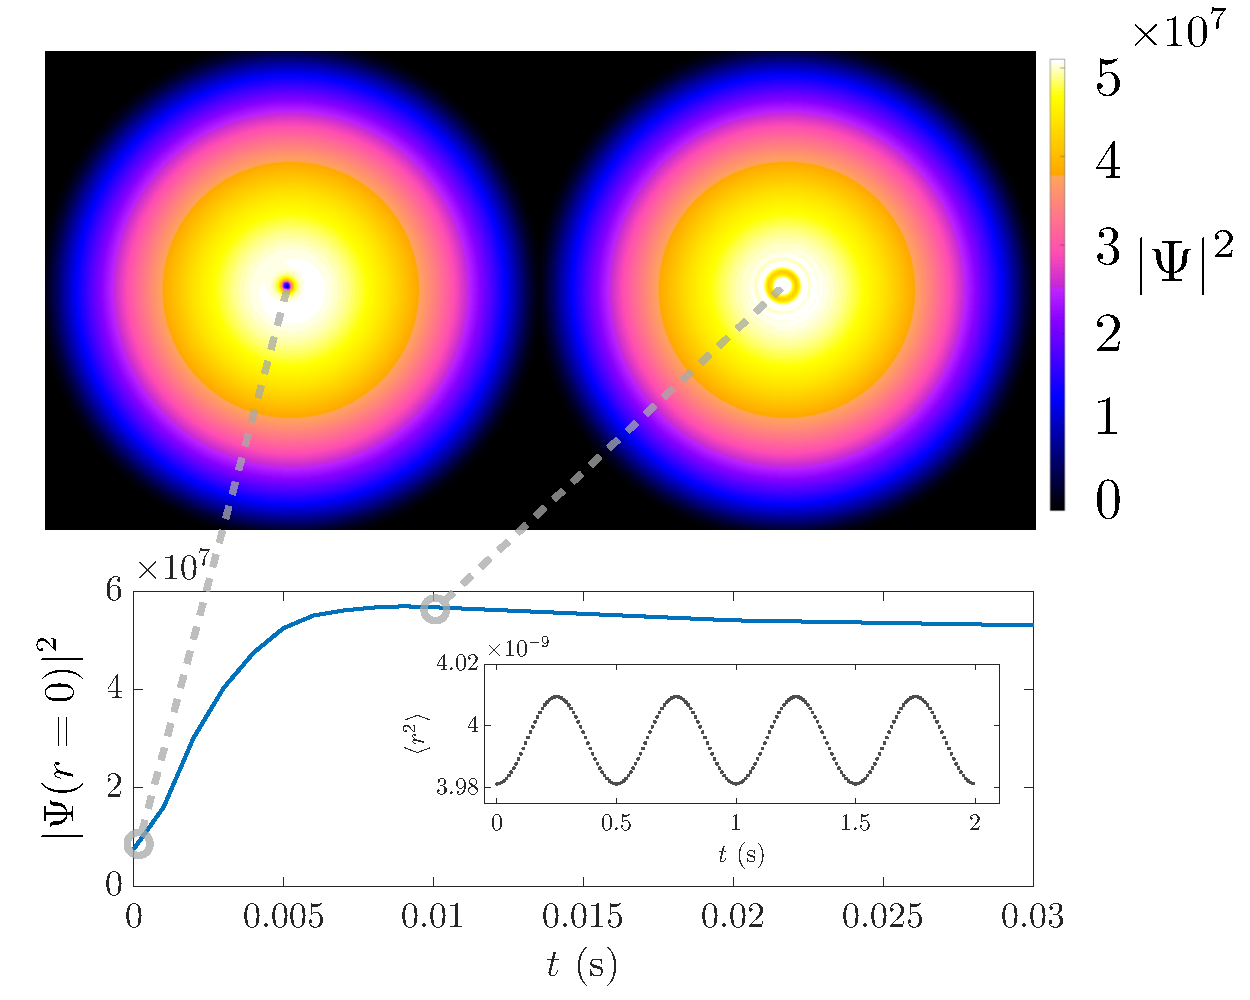
\includegraphics[width=0.55\textwidth, angle=0, trim=0 0 0 0]{ch5_kickit/fig1}
    \caption[Comparison of vortex lattice and optical lattice structures.]{(a) Vortex lattice ground-state in a harmonic trap with $\omega_\perp=2\pi$ s$^{-1}$ and rotating at $\Omega=0.995\omega_\perp$. This plot shows a condensate with a diameter of approximately $580~\mu\textrm{m}$; (b) Zoom in of vortex lattice at central density; (c) Optical lattice potential with a periodicity matching that of the vortex lattice.}
    \label{fig:vlatt_gnd}
\end{figure}

Given the large number of vortices in the condesate density, as well as the lowered density resulting from large centrifugal forces, the vortex cores become large and form a highly periodic triangular lattice. The non-orthogonal lattice vectors are given in $\mathbf{r}$-space by $\mathbf{a}_1 = a_v\{1,0\}$ and $\mathbf{a}_2 = a_v\{-1/2, \sqrt{3}/2\}$, where $a_v$ is the distance between vortex cores. The lattice ``constant'' is truly only constant in areas of near uniform density. Thus, due to the inhomogeneous wavefunction density, the vortices near the edges are separated by a much greater distance than those at the centre. For my analysis I have chosen to ignore all vortices near the condensate edge. The momentum space ($\mathbf{k}$-space) lattice vectors reciprocal to the given $\mathbf{r}$-space vectors are $\mathbf{b}_1 = 4\pi/(\sqrt{3}a_v)\{\sqrt{3}/2,1/2\}$ and $\mathbf{b}_2 = (4\pi/(\sqrt{3}a_v))\{0,1\}$.

Using an optical potential one can create a perturbation in the condensate density by switching it on for a brief period of time. Such a {\it kick} must occur only for a time much shorter than the rotation period of the vortex lattice, $\Omega = 0.995\omega_\perp$. For the work carried out herein, the time of the kick was given by $\tau_{\text{kick}}=10^{-5}$~s. This ensured that the vortex lattice was essentially stationary during the kick. To examine the effect that periodicity plays on the system, the optical potential was chosen to match the structure of the Abrikosov vortex lattice, with the angle of relative rotation $\theta_\Delta$ given as a free parameter. The optical potential was modeled as the sum of counter-propagating laser beams, as
\begin{equation}
    V_{\text{opt}} = V_0\displaystyle\sum_{j}\cos^2 \left[ \textbf{k}_{j}\cdot\textbf{r} \right],
\end{equation}
where $V_0$ is the optical lattice potential amplitude, and $j=\lbrace 0,1,2,\ldots \rbrace$ is the index of each respective laser with a differing $\mathbf{k}$-space wave-vector. By careful choice of the wave-vectors $\textbf{k}_{j}$ the density modulation given by the vortices is matched to the optical potential. This is achieved using the reciprocal lattice vectors defined by the vortex lattice, $\mathbf{b}_{1,2}$, and an additional third wave-vector, $\mathbf{k}_3 = 4\pi/(\sqrt{3}a_o)\{\sqrt{3}/2,-1/2\}$. The lattice constant of the resulting potential is based on the optical intensity to match that of the vortex lattice.


As the vortex lattice constant in a rapidly rotating atomic BEC is large, optical lattices with wavelengths on the order of tens of microns are necessary \cite{BEC:Fallani_optexp_2005, AO:Williams_optexp_2008}. By ensuring a short kick with an amplitude on the order of $10^{-2} \mu $, with $\mu$ as the BEC chemical potential, the result of the kick is an imprinted phase on the wavefunction \cite{Vtx:Dobrek_pra_1999}. This leads to the development of a flow from the origin of each optical lattice potential maxima, and creates well-defined interference patterns resulting from phonons created by the kick. In the presence of a vortex lattice with a periodic core arrangement, this creates moir\'e superlattice structures \cite{SS:Murata_acsn_2010} in the density of the condensate. Although this type of pattern has been observed in many solid-state systems, such as graphene on hexagonal boron nitride~\cite{SS:Yankowitz_natphys_2012}, they appear to be static in such cases. In this system, the structures are dynamical, and revive at well defined intervals.

To study these resulting structures, I performed a spectral decomposition of the kinetic energy of the condesate~\cite{CT:Nore_prl_1997,CT:Nore_pof_1997,CT:Bradley_prx_2012}. For this the wavefunction is first written in amplitude (density) $\rho(\mathbf{r},t)$ and phase $S(\mathbf{r},t)$ form via a Madelung transform as given by \ref{eqn:madelung}.
\iffalse
as
$
		\Psi(\mathbf{r},t) = \sqrt{\rho(\mathbf{r},t)}\exp{\left[\mathrm{i}S(\mathbf{r},t)\right]}.
$
\fi
Making use of the Gross--Pitaevskii energy functional \ref{eqn:gpe_functional}, and substituting in the above form gives
\begin{equation}
    E_{\text{kqp}} = \int d\mathbf{r} \left( \frac{\hbar^2}{2m}| \nabla\sqrt{\rho(\mathbf{r},t)} |^2  + \frac{m}{2}|\sqrt{\rho(\mathbf{r},t)}\mathbf{v}(\mathbf{r},t) |^2\right).
\end{equation}
One can decompose this into the quantum pressure (first) and kinetic energy (second) terms. The kinetic energy term can seen as a density-weighted velocity field, $\mathbf{u}(\mathbf{r},t) = \sqrt{\rho(\mathbf{r},t)}\mathbf{v}(\mathbf{r},t)$. This can be further decomposed into the sum of compressible and incompressible terms,
\begin{equation}
    \mathbf{u(r},t) = \mathbf{u}^c(\mathbf{r},t) + \mathbf{u}^i(\mathbf{r},t),
\end{equation}
where $\mathbf{u}^c, \mathbf{u}^i$ are the compressible and incompressible terms respectively. These can be solved by assuming $\nabla \times \mathbf{u}^c(\mathbf{r},t) = 0$, and $\nabla \cdot \mathbf{u}^i(\mathbf{r},t) = 0$. This decomposition separates the energy contribution from phonons and vortex cores, representing compressible and incompressible terms respectively~\cite{CT:Horng_pra_2009}. By averaging over binned shells in $\mathbf{k}$-space, the kinetic energy spectra, $E^{c,i}(k)$, are calculated as~\cite{CT:Bradley_prx_2012}
\begin{equation}
	E^{c,i}(k) = \frac{mk}{2}\sum\limits_{j\in\mathbf{r}} \int\limits_{0}^{2\pi}d\phi_k \frac{ |\mathcal{U}_j^{c,i}(\mathbf{k},t) |^2}{s_k},
\end{equation}
where
\begin{equation}
	\mathcal{U}_j^{c,i}(\mathbf{k},t) = \int d^2 \mathbf{r} e^{-i(\mathbf{k}\cdot\mathbf{r})} u_j^{c,i}(\mathbf{r},t).
\end{equation}
The terms $u_j^{c,i}(\mathbf{r},t)$ represent the position-space density-weighted velocity components in the specified shell, where $\phi_k$ is the polar angle, and $s_k$ is the number of values in the chosen shell.

For a rapidly rotating vortex lattice carrying condensate, calculating the spectra via the above method returns quantities which closely resemble those used in classical fluid calculations. Such an example can be seen in Fig. \ref{fig:ek_clvqu}. However, Reeves {\it et al} [PHYS. REV. A 89, 053631 (2014)] have discussed how this method does not truly represent the kinetic energy of the system, as the decomposed spectra terms are not additive in $k$-space. The classical interpretation is described as being ``obtained by applying the general correspondence between a two-point correlation function and its associated
power spectrum to the velocity field'', as stated by the authors. They propose a quantum version of the above description, which involves including the condensate phase, alongside the density weighted velocity field, as $\mathbf{u}(\mathbf{r},t) = \sqrt{\rho(\mathbf{r},t)}\mathbf{v}(\mathbf{r},t)\exp\left(iS(\mathbf{r},t)\right)$. The inclusion of a quantum phase term essentially destroys the correspondence in the classical case. The resulting kinetic spectra may now accurately describe the true spectrum of the condensate, however, the structure observed in the classical spectra are lost, which were reminiscent of a two-body correlation function, as seen in Fig. \ref{fig:ek_clvqu}. The effect of kicking on the kinetic terms can be observed in the compressible spectrum in both cases, and thus, the work described will use the ``classical'' method herein to allow observable peaks to be easily examined.

\begin{figure}[tb]
    \centering
    \includegraphics[width=0.45\textwidth,trim=0 0 0 0,clip=true]{ch5_kickit/Ek_classical/VTXLATT_Ek.png}
    \includegraphics[width=0.45\textwidth,trim=0 0 0 0]{ch5_kickit/Ek_quantum/VTXLATT_Ek.png}

    \includegraphics[width=0.45\textwidth,trim=0 0 0 0,clip=true]{ch5_kickit/Ek_classical/VTXLATT_Comp.png}
    \includegraphics[width=0.45\textwidth,trim=0 0 0 0]{ch5_kickit/Ek_quantum/VTXLATT_Comp.png}

    \includegraphics[width=0.45\textwidth,trim=0 0 0 0,clip=true]{ch5_kickit/Ek_classical/VTXLATT_Incomp.png}
    \includegraphics[width=0.45\textwidth,trim=0 0 0 0]{ch5_kickit/Ek_quantum/VTXLATT_Incomp.png}

\caption[Kinetic energy spectra with and without quantum phase.]{The kinetic energy spectra (T), compressible (M), and incompressible energies (B), comparing the classical (L) and the quantum version (R). The inclusion of the phase term eliminates the peaks from the compressible energy, yet yields a more accurate representation of the magnitude of both energies.}
\label{fig:ek_clvqu}
\end{figure}


\section{Delta-kick dynamics}\label{sec:kickvl}
\subsection{Non-rotating condensate}
To fully characterise the effect kicking has on a rapidly rotating BEC carrying a vortex lattice it is instructive to understand the dynamics following a kick in the absence of a vortex lattice. For an accurate comparison, the trapping frequency of the non-rotating condensate is adjusted such that the background densities match that of the rotating condensate. This is achieved by assuming the centrifugal term competing against the harmonic oscillator frequency as $V_{\text{opt}} = 1/2m(\omega^2_\perp - \Omega^2)\mathbf
{r}^2$, where $\Omega=0.995\omega_\perp$ is the value chosen for the rapidly rotating case.

For a stationary (non-kicked) condensate the kinetic energy spectrum will remain constant during time-evolution, with a kick leading to the appearance of new, time varying components. To observe this I numerically evolve the system by setting $V(\mathbf{r},t) = V_{\text{ext}}(\mathbf{r}) + V_{\text{opt}}(\mathbf{r},t)$, where the time dependent optical potential is only active for $\tau=10^{-5}$~s of the simulation time. As discussed earlier, this short kicking duration is sufficient to allow a phase imprint onto the condensate wavefunction, without any change in the density on the timescales of the kick itself. Next, I examine the compressible and incompressible kinetic energy spectrum following the kick (see Fig.~\ref{fig:ekc_eki_novtx}). Unsurprisingly, the spectrum is dominated by a peak corresponding to the wave-number associated with the optical potential at $k=4\pi/(\sqrt{3}a_o)$, and several smaller ones corresponding to higher harmonics of $n$-th next nearest neighbour components of the lattice. This makes sense as the nearest neighbour lattice spacings should be the dominant structure with higher order spacings dropping in intensity due to the finite system size. As no rotation is added by the imparted phonon modes, the incompressible energy is an order of magnitude smaller compared to the compressible energy \ref{fig:ordermagsmaller}. Following from this I will restrict the analysis to the compressible part of the spectrum.

\begin{figure}[tb]
    %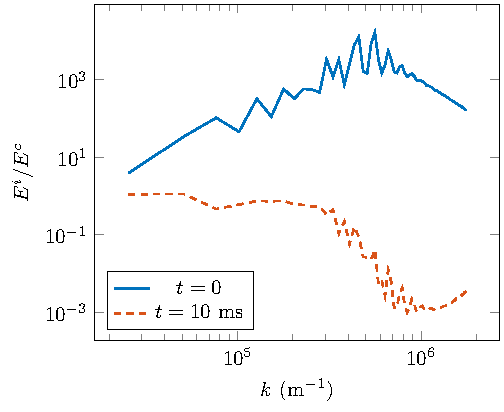
\includegraphics[width=0.48\textwidth]{ch5_kickit/fig2}
    \centering
    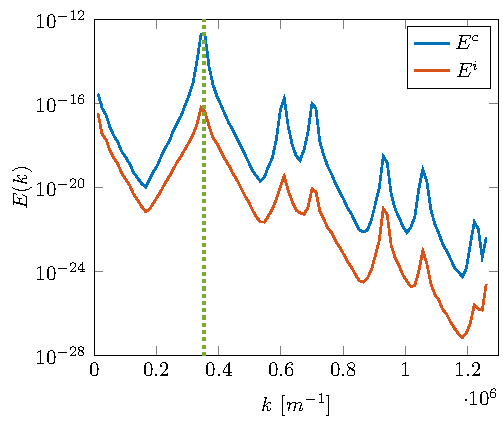
\includegraphics[width=0.55\textwidth]{ch5_kickit/EKcEKi_kick_dt2}
    \caption[Time-averaged compressible and incompressible energy spectra of a non-rotating condensate directly following a kick.]{Compressible and incompressible energy spectra of a non-rotating condensate directly following a kick. A peak at $k=4\pi/(\sqrt{3}a_o)$ can be seen, which corresponds to the lattice spacing, $a_o$ (indicated by the dashed line), and the smaller, higher energy peaks can be attributed to higher harmonics between nearest and next-nearest neighbours. The incompressible spectrum is much smaller than the compressible spectrum, and thus is neglected for all further analysis.}
    \label{fig:ekc_eki_novtx}
\end{figure}


The evolution of the nearest neighbour peak in the compressible kinetic energy spectrum during the first 250 ms after the kick is shown in Fig.~\ref{fig:novtx_p5k}(a). It initially oscillates in and out of existence and eventually disperses over a wide range of wave-numbers. Snapshots of the density evolution are given in Fig.~\ref{fig:novtx_p5k}(b), which clearly show that the oscillations correspond to the existence of a transient lattice pattern with several revivals, having the same underlying structure as the optical potential. In fact, the lattice pattern is best formed whenever the main peak in the kinetic energy spectrum goes to zero, i.e.~when the imprinted kinetic energy has been converted into density modulations. The period of the oscillations can be related to the speed of sound divided by the lattice constant and therefore the appearance of the lattice can be attributed to phonon interference.

\begin{figure}[tb]
    \centering

	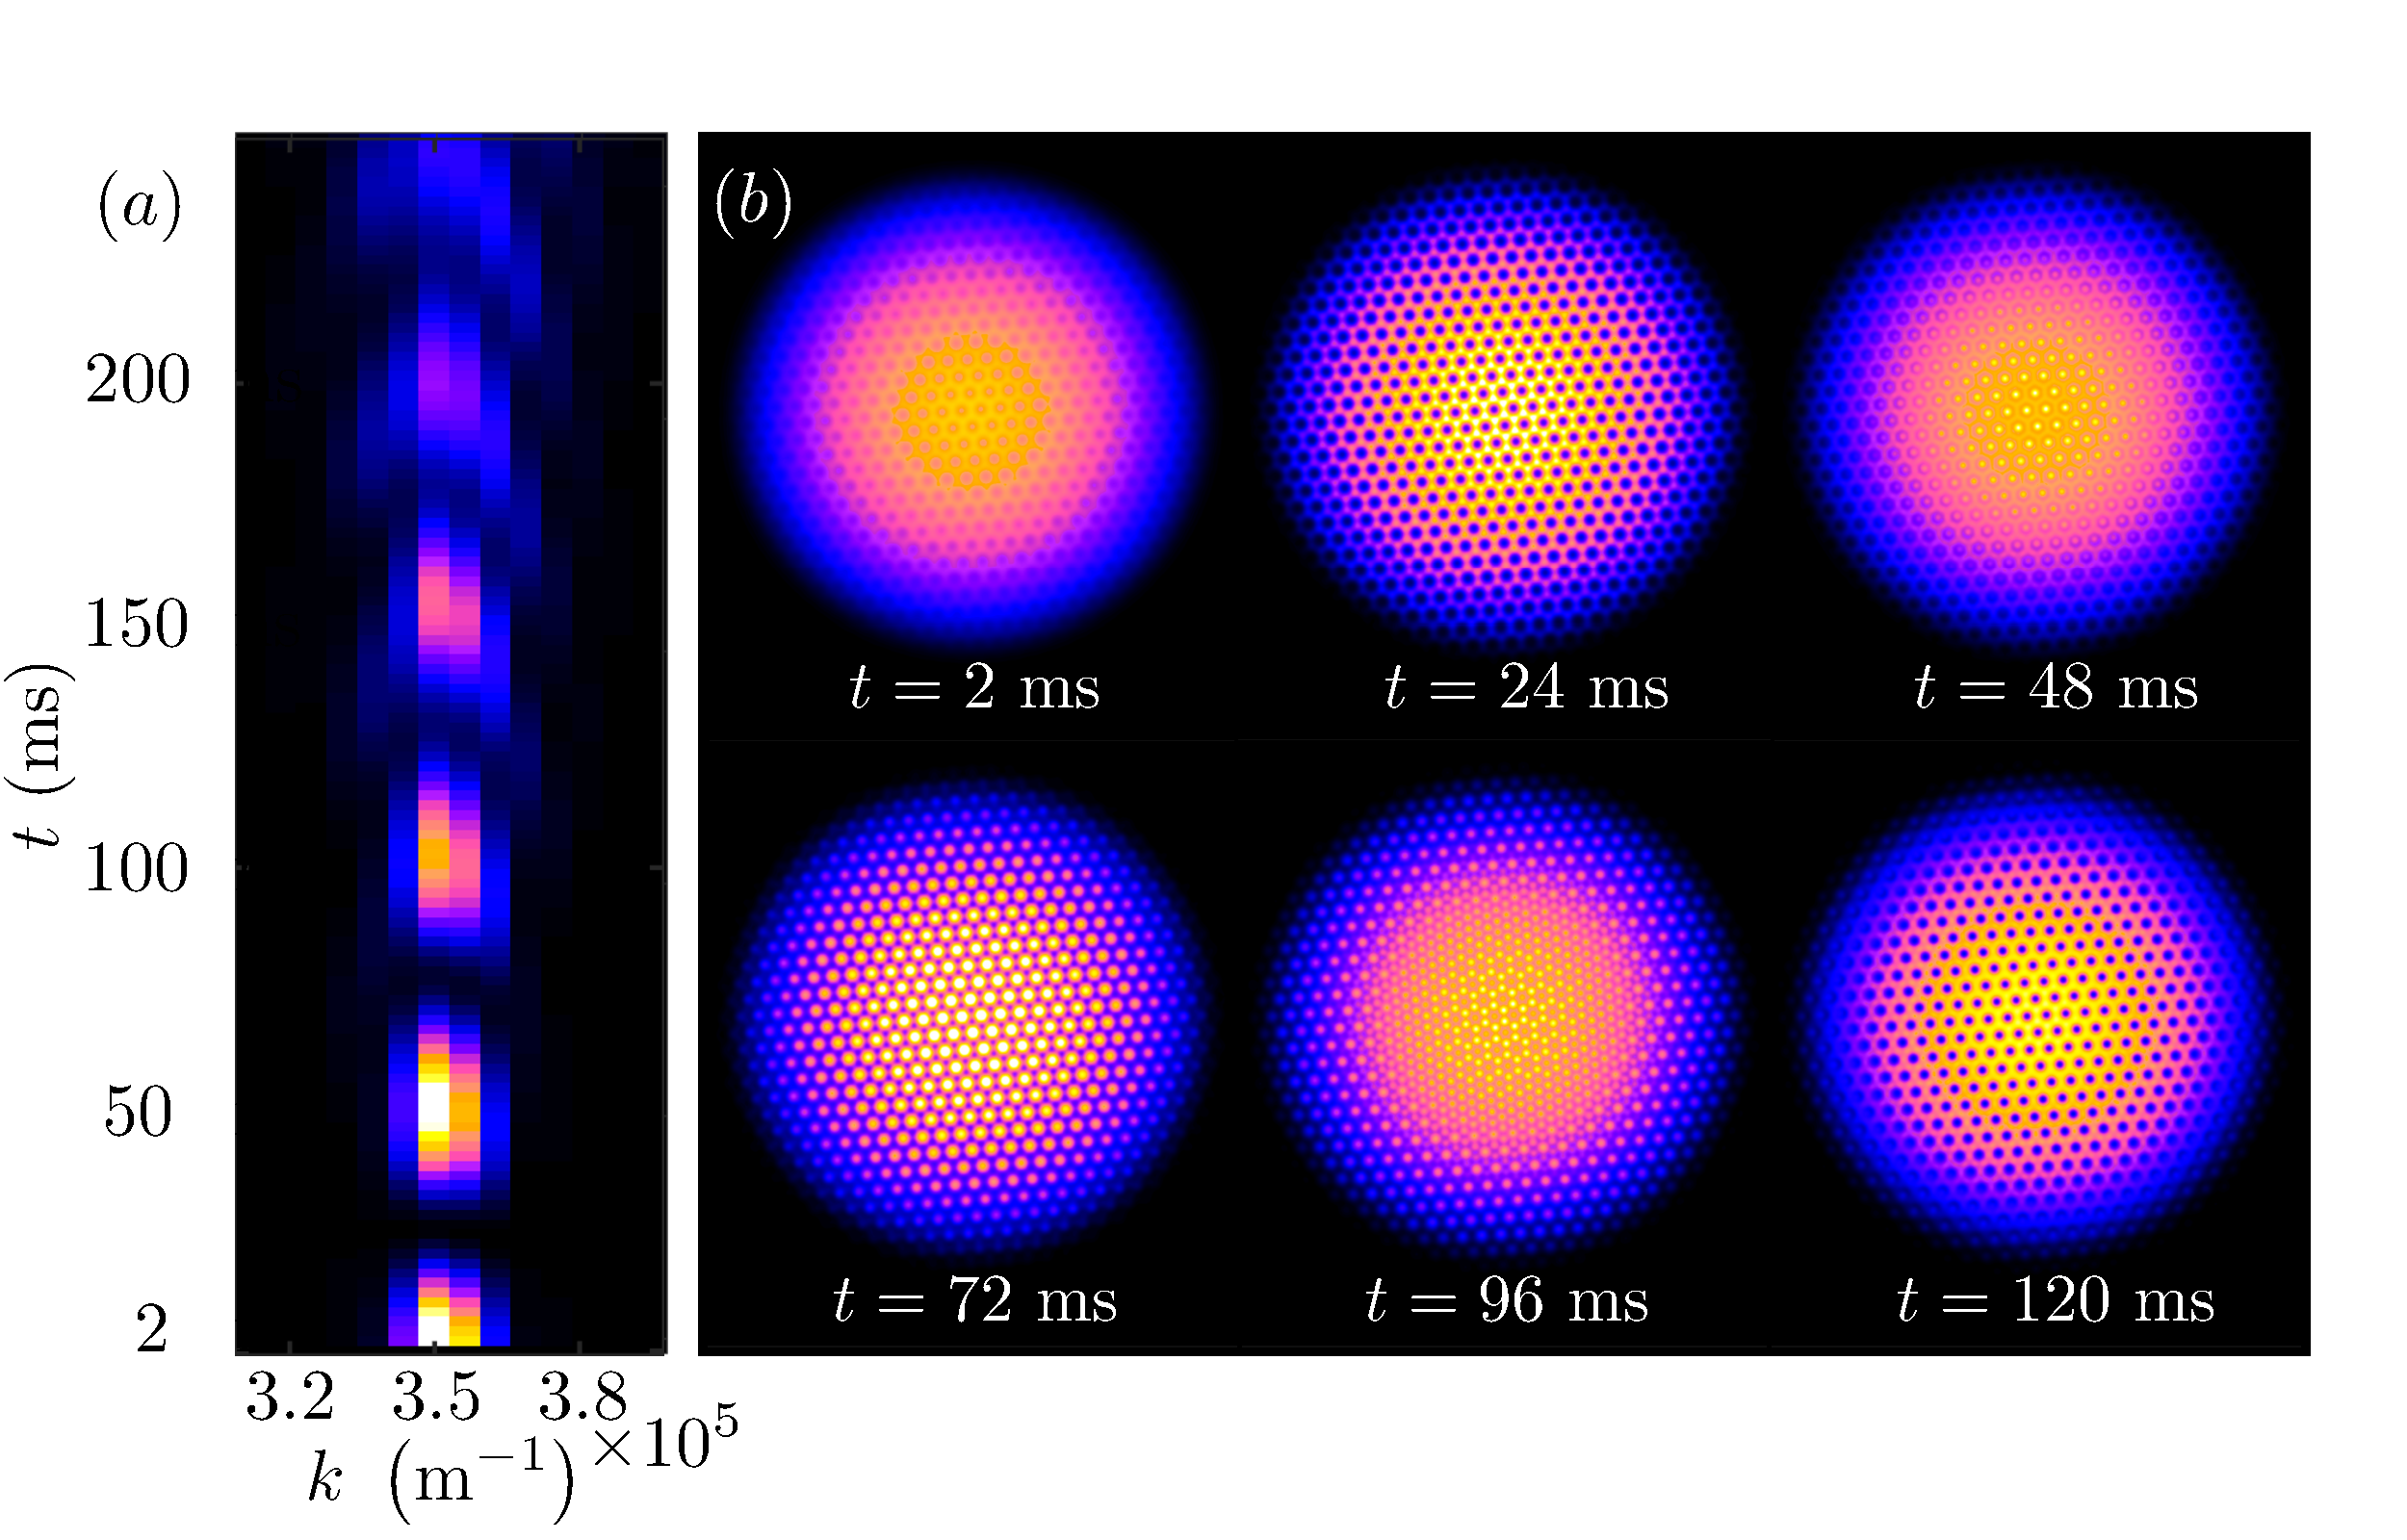
\includegraphics[width=0.55\textwidth]{ch5_kickit/fig3}
	\caption[Effect of kicking on non-rotating condensate.]{(a) Main peak of the compressible kinetic energy spectrum for a kicking strength of $V_0 \approx 1.35\times10^{-2}\mu$. It can be seen to revive, and eventually disperse over a wide range of wave-numbers.  (b) Condensate densities at several times during the evolution. A pattern matching the optical potential can be observed to appear and disappear several times over the course of the evolution.}
	\label{fig:novtx_p5k}
\end{figure}


%######################################################%#################################################################################%############################################################################################################
\subsection{Rapidly rotating condensate}

    Kicking a condensate carrying an Abrikosov vortex lattice with the above optical lattice gives an additional parameter, $\theta_\Delta$, which describes the orientation of the imprinted phonon lattice angle relative to the vortex lattice. For simplicity, it is assumed that the vortex and optical potential lattices have the same lattice constant, $a_v=a_o=a$ (see below for a discussion of the incommensurate case), which means that symmetry allows us to restrict the angle to $\theta_\Delta\in[0,\pi/3]$. In the following it can be seen that adjusting $\theta_\Delta$ leads to the appearance of different, transient super-structures in the condensate density.

    If $\theta_\Delta=0$ (see Fig.~\ref{fig:moire_density}(a)) the kicking imparts kinetic energy at wave-numbers that are already well defined in the lattice. Provided that the optical lattice makes contact with some non-zero density region their cores will expand and contract with oscillations in the density. No significant change to the compressible kinetic energy spectrum is observed in this case, apart from small amplitude modulations on the well defined peaks.

	\begin{figure}[tb]
        \centering
			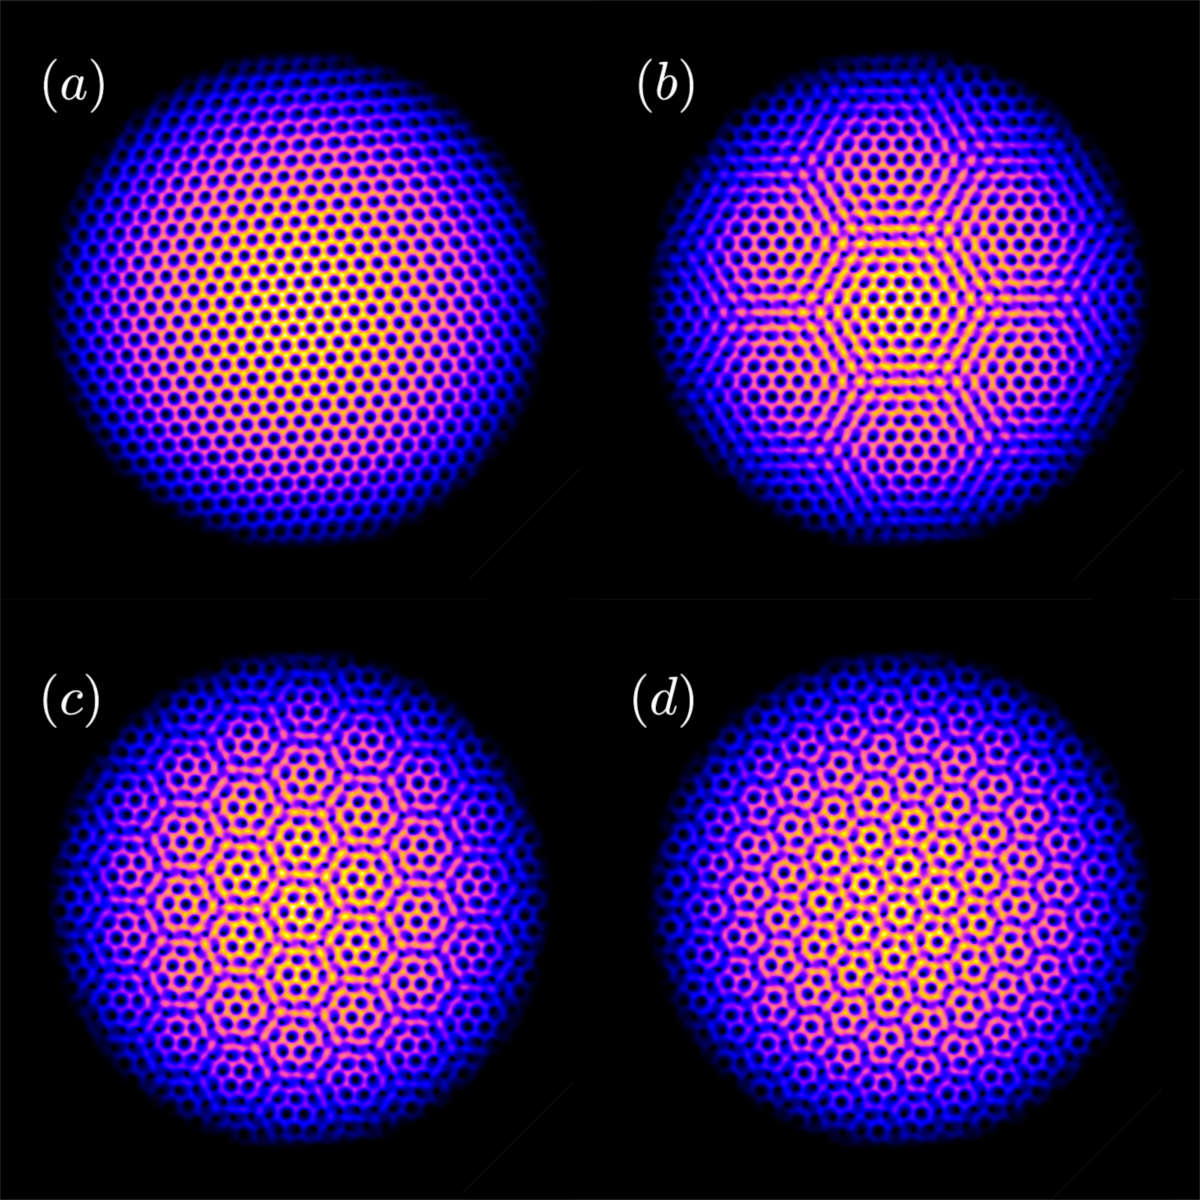
\includegraphics[width=0.55\textwidth]{ch5_kickit/fig4}
			\caption[Effect of kicking on condensate with a large vortex lattice.]{Condensate density at $t=1.4\times10^{-2}$ s for several optical lattice rotation angles. The cell size of the super-lattice structures can be seen to shrink as the angle is increased. The angles for the examples shown are $(a)~\theta_\Delta=0$, $(b)~\theta_\Delta=2\pi/45$, $(c)~\theta_\Delta=4\pi/45$, $(d)~\theta_\Delta=2\pi/15$. }
			\label{fig:moire_density}
		\end{figure}

    However, if the angle between both lattices is finite, and not an integer multiple of $\pi/3$, superlattice structures appear after a short time (see Fig.~\ref{fig:moire_density}(b)-(d)), which have a structure cell size that decreases for increasing values of $\theta_\Delta\in[0,\pi/6]$ and beyond which increases for larger values until the misalignment angle reaches the lattice symmetry point again at $\theta_\Delta=\pi/3$. These structures are transient, and several revivals can be observed before the condensate settles back into the vortex lattice structure with an increase in the background wave-number spread, as expected based on kicking the non-rotating condensate. An example of this for a fixed angle is shown in Fig.~\ref{fig:dtheta20_ev}. It is expected that with dissipation this would return to the perfect Abrikosov lattice, with no background increase of wave-numbers.

	\begin{figure}[bt]
        \centering
		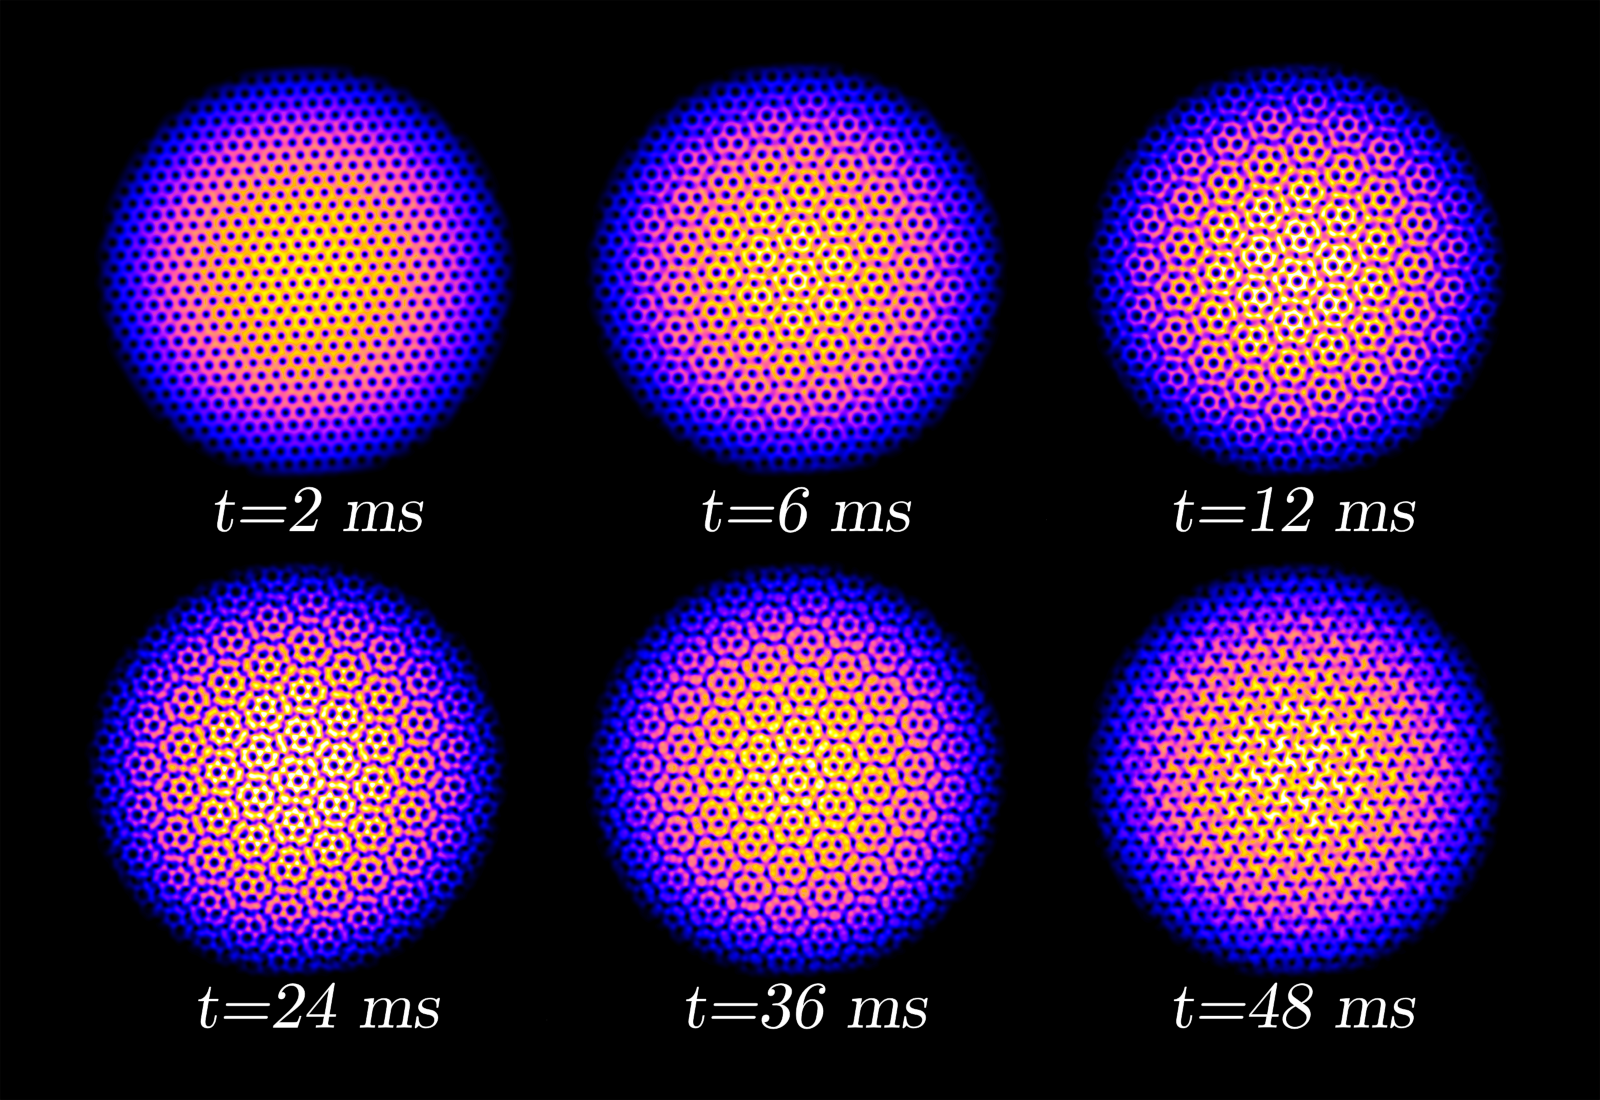
\includegraphics[width=0.55\textwidth]{ch5_kickit/fig5}
		\caption[Oscillation of moir\'e wavelength.]{Condensate density shows visible moir\'e structures upon receiving a kick with $\theta_\Delta=\pi/9$. The appearance and disappearance of a moir\'e structure with wavelength $\lambda_M \approx 2.9 a$ over a timescale of about $50$ ms can be seen.}
		\label{fig:dtheta20_ev}
	\end{figure}

    To explain the interference patterns observed for misaligning the optical and the vortex lattice, I employ moir\'e interference theory \cite{SS:Hermann_jpcm_2012}. Moir\'e patterns are known to appear when two periodic structures are overlaid while slightly misaligned to each other, and can be calculated from the reciprocal lattice vectors. In all generality, any choice of equidistantly separated reciprocal lattice vectors can be parameterised as
    	\begin{equation}
    		\mathbf{g}_{l} = g_0 \left[ \sin\left( \frac{2\pi l}{\alpha}+\theta \right),\, \cos\left( \frac{2\pi l}{\alpha} +\theta\right) \right],
    	\end{equation}
    where $\alpha$ describes the rotational symmetry of the lattice, $l$ labels the vector direction on the unit circle, $\theta$ is the angle with respect to a chosen coordinate system and $g_0$ is the reciprocal lattice constant. For a commensurate and triangular lattices we get $g_0=4\pi/(\sqrt{3}a)$, $\alpha=6$ and the vector directions are $l=\left[0\dots\alpha-1\right]$. As only the relative mis-alignement between the vortex and the phonon lattice matters, I choose $\theta=0$ for the vortex lattice and $\theta=\theta_\Delta$ for the optical potential alignment.
    All possible wavelengths that can appear in an interference pattern between two such lattices in real space are then given by
    	\begin{equation}
    		\lambda_{ll'} = \frac{\lambda_0}{|\mathbf{\mathbf{g}_{ll'}|}},
    		\label{eq:InterferenceVectors}
    	\end{equation}
    where
    $\mathbf{g}_{ll'}=\mathbf{g}_{l}^{\text{V}}-\mathbf{g}_{l'}^{\text{P}}$, and
    $\lambda_0 = 4\pi/\sqrt{3}$ for the commensurate triangular lattices.
    One can see from Fig.~\ref{fig:dtheta20_ev} that a pattern matching the longest wavelength, $\lambda_M= \max[\lambda_{ll'}] \approx 2.9 a$, appears around $t=24$~ms and is clearly the most visible one for the given angle. While patterns with shorter wavelength exist, they are harder to discern in this system and therefore I concentrate on the lowest wave-number in the following. It should be noted that given sufficient time the higher order wave-numbers do influence the density dynamics, but the system remains dominated by the lowest wave-number. Due to coupling between adjacent modes in the system, all interference patterns tend to become hard to discern after some time. It is expected (but not investigated) that in the long time limit the interference patterns will eventually refocus and reappear.

    In $\mathbf{k}$-space the shortest $|\mathbf{g}_{ll^\prime}|$ corresponds to adjacent wave-vectors with the smallest $\theta_\Delta$ between them (see inset in Fig.~\ref{fig:moire_lambda_1}). Due to the symmetry of the lattices the most visible structures are therefore given by $\lambda_M=\lambda_{00}$ for $\theta_\Delta\in[0,\pi/6]$ and $\lambda_M=\lambda_{01}$ for $\theta_\Delta\in[\pi/6,\pi/3]$ (see inset of Fig.~\ref{fig:moire_lambda_1}).
    While this symmetry assumption no longer holds strictly true after the system has been kicked, it is still fulfilled to a very good approximation during the initial dynamics. One can then obtain the wavelength of the dominating moir\'e structure as~\cite{BIO:Blair_jneur_2007,SS:Yankowitz_natphys_2012}
    		\begin{equation}
    		\lambda_M = \frac{a}{2\sin(\eta/2)},
    		\label{eqn:moire_size}
    	\end{equation}
    where $\eta=\min\{\theta_\Delta,\frac{\pi}{3} - \theta_\Delta \} $  (see Fig.~\ref{fig:moire_lambda_1}).
These super-structures become observable when the wavelength becomes smaller than the radius of the condensate, which for the chosen parameters is $\lambda_M \approx 11a$ and which corresponds to an angle $\theta_\Delta \approx \pi/36$.
One can see from Fig.~\ref{fig:moire_lambda_1} that once the relative angle is increased beyond this value the structure sizes shrink to a minimum value at the point of complete misalignment, $\theta_\Delta=\pi/6$, giving $\lambda_M\approx 1.93\,a$, and increase again up to the point of symmetry. Beyond this point the behaviour starts over, due to the symmetry of the lattice. Note that in principle the above procedure can be carried out for square or other optical lattice geometries.

\begin{figure}[tb]
    \centering

	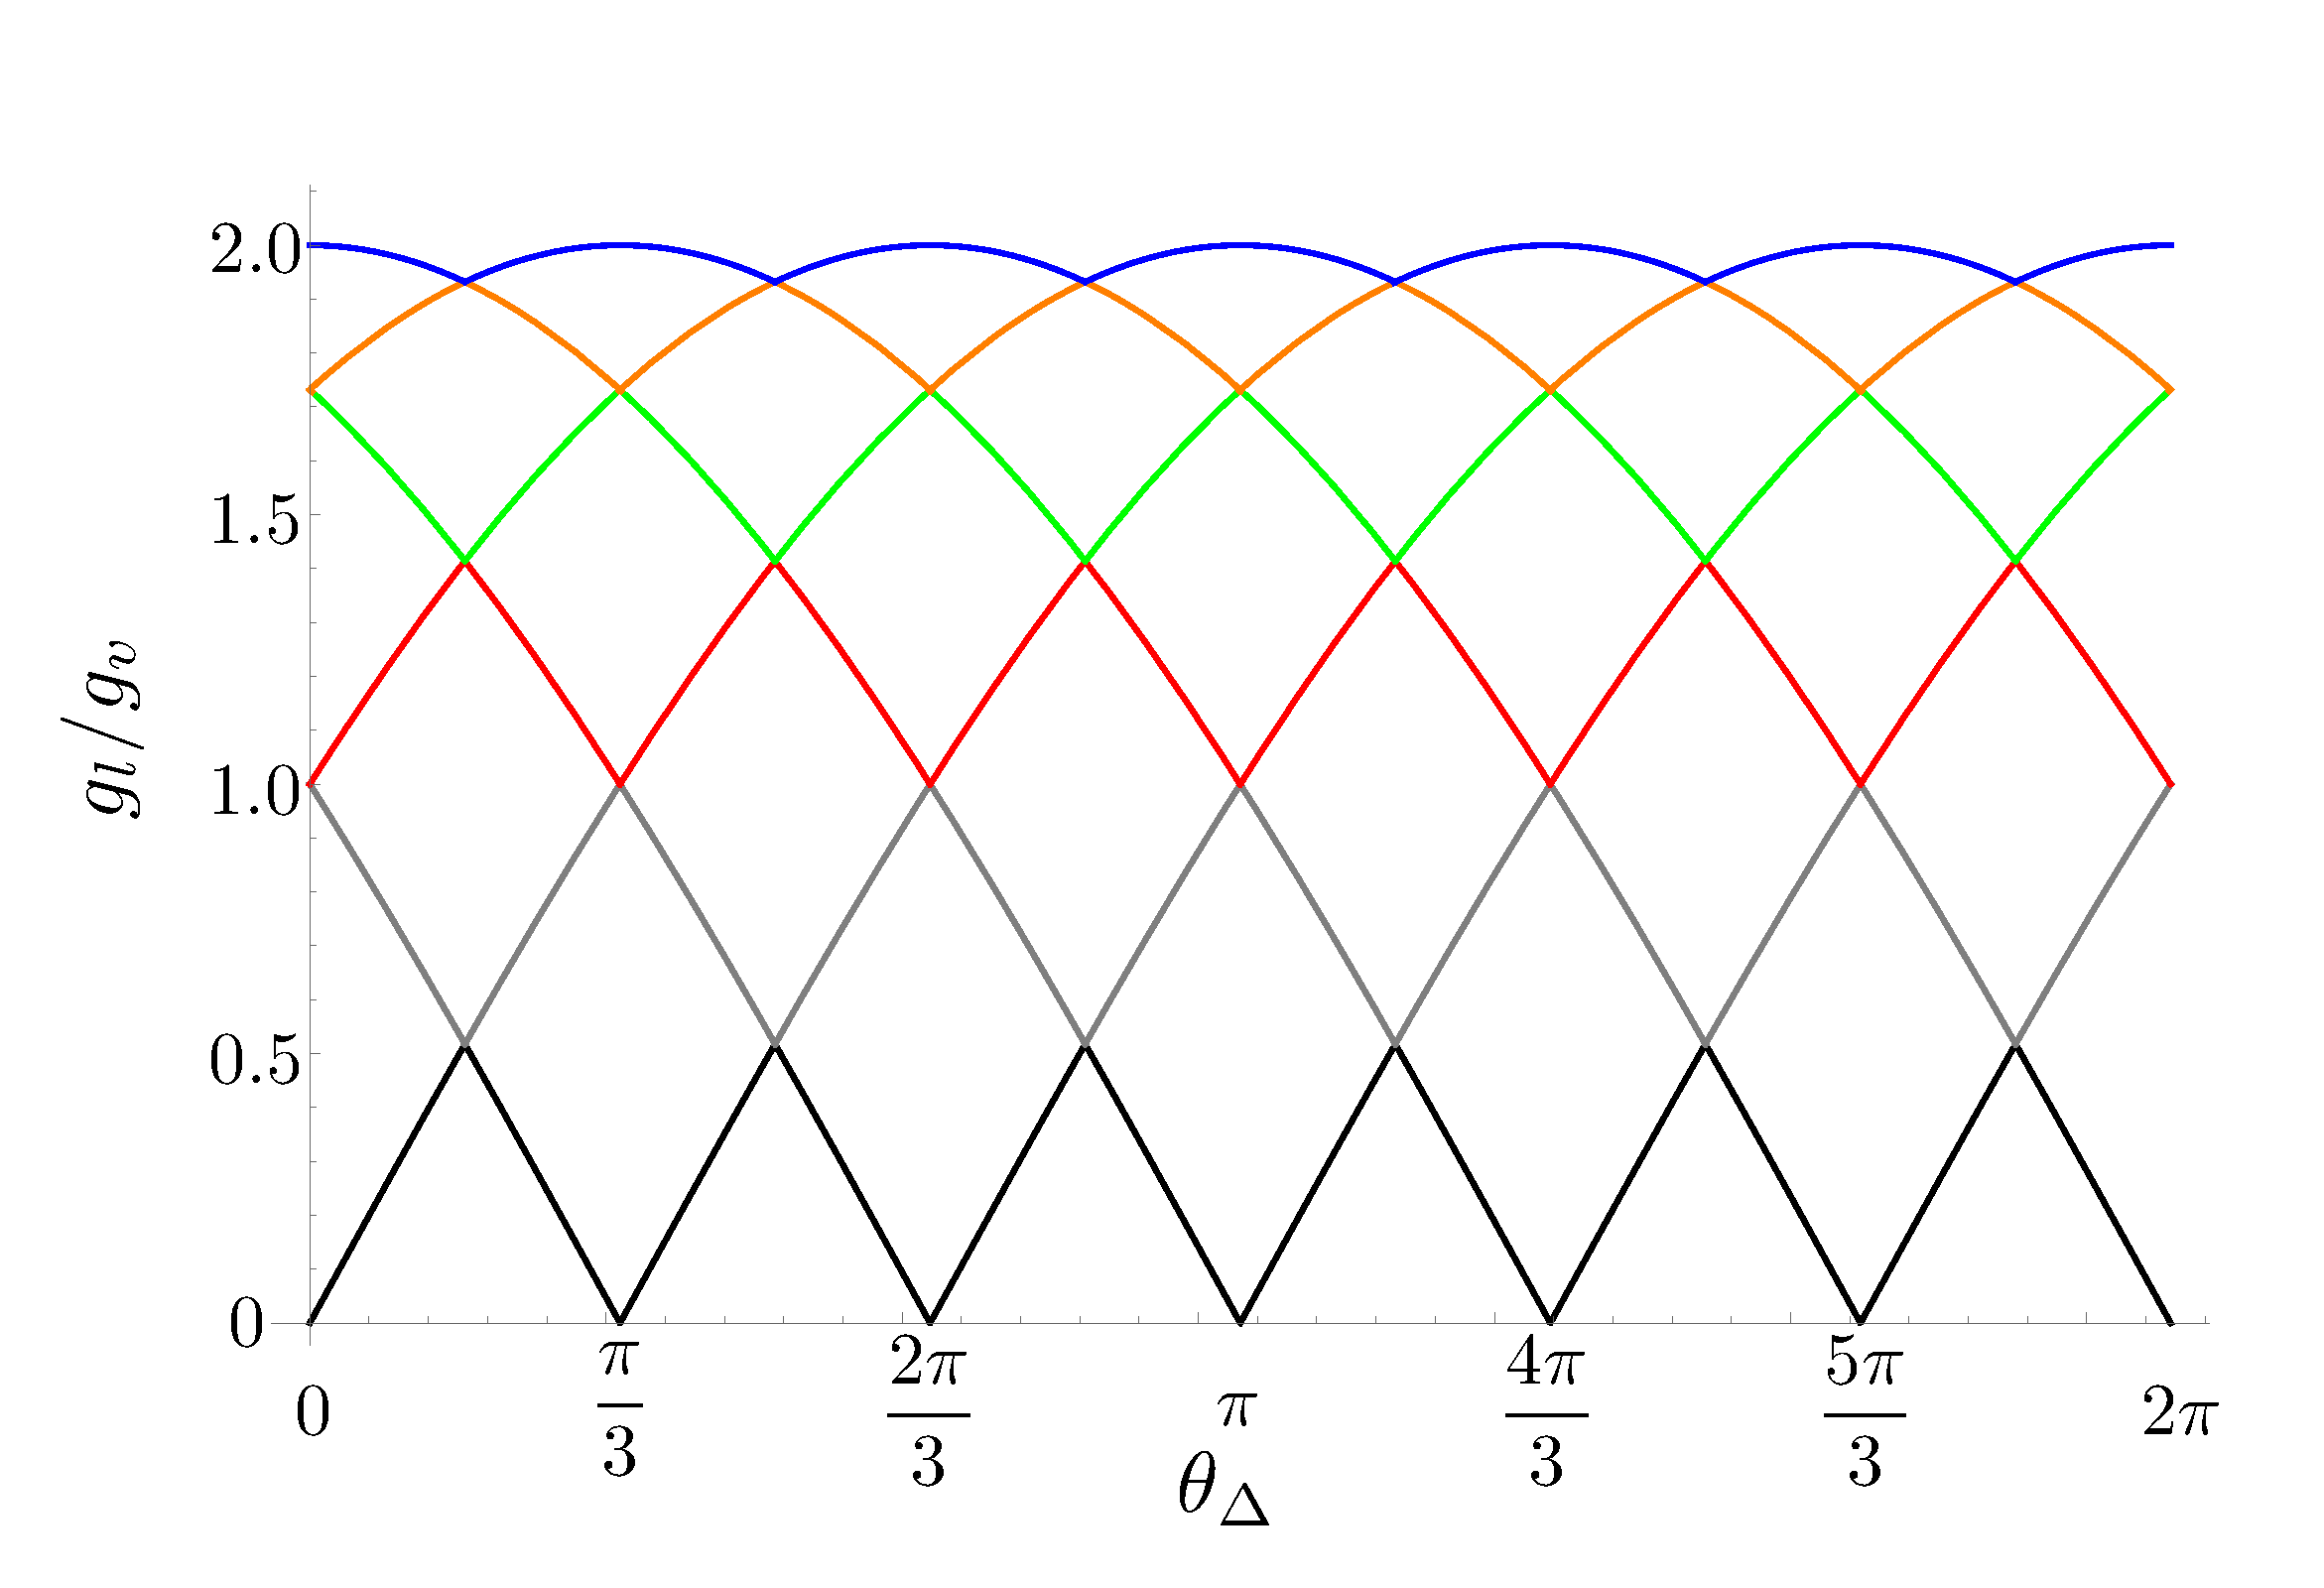
\includegraphics[width=0.55\textwidth]{ch5_kickit/Moire_lattice_BEC_HigherK_lambda}
    \caption[The moir\'e interference pattern in terms of wavenumbers.]{The moir\'e interference pattern in terms of wavenumbers. The resulting wavenumber $g_l$ is normalised by the vortex lattice spacing in reciprocal space $g_v$. The lowest lying (black) band is the main contributor to the dynamics of the moir\'e interference pattern, with higher modes mostly visible between beats of lowest wave-number moir\'e only.}
\end{figure}



\begin{figure}[tb]
    \centering

	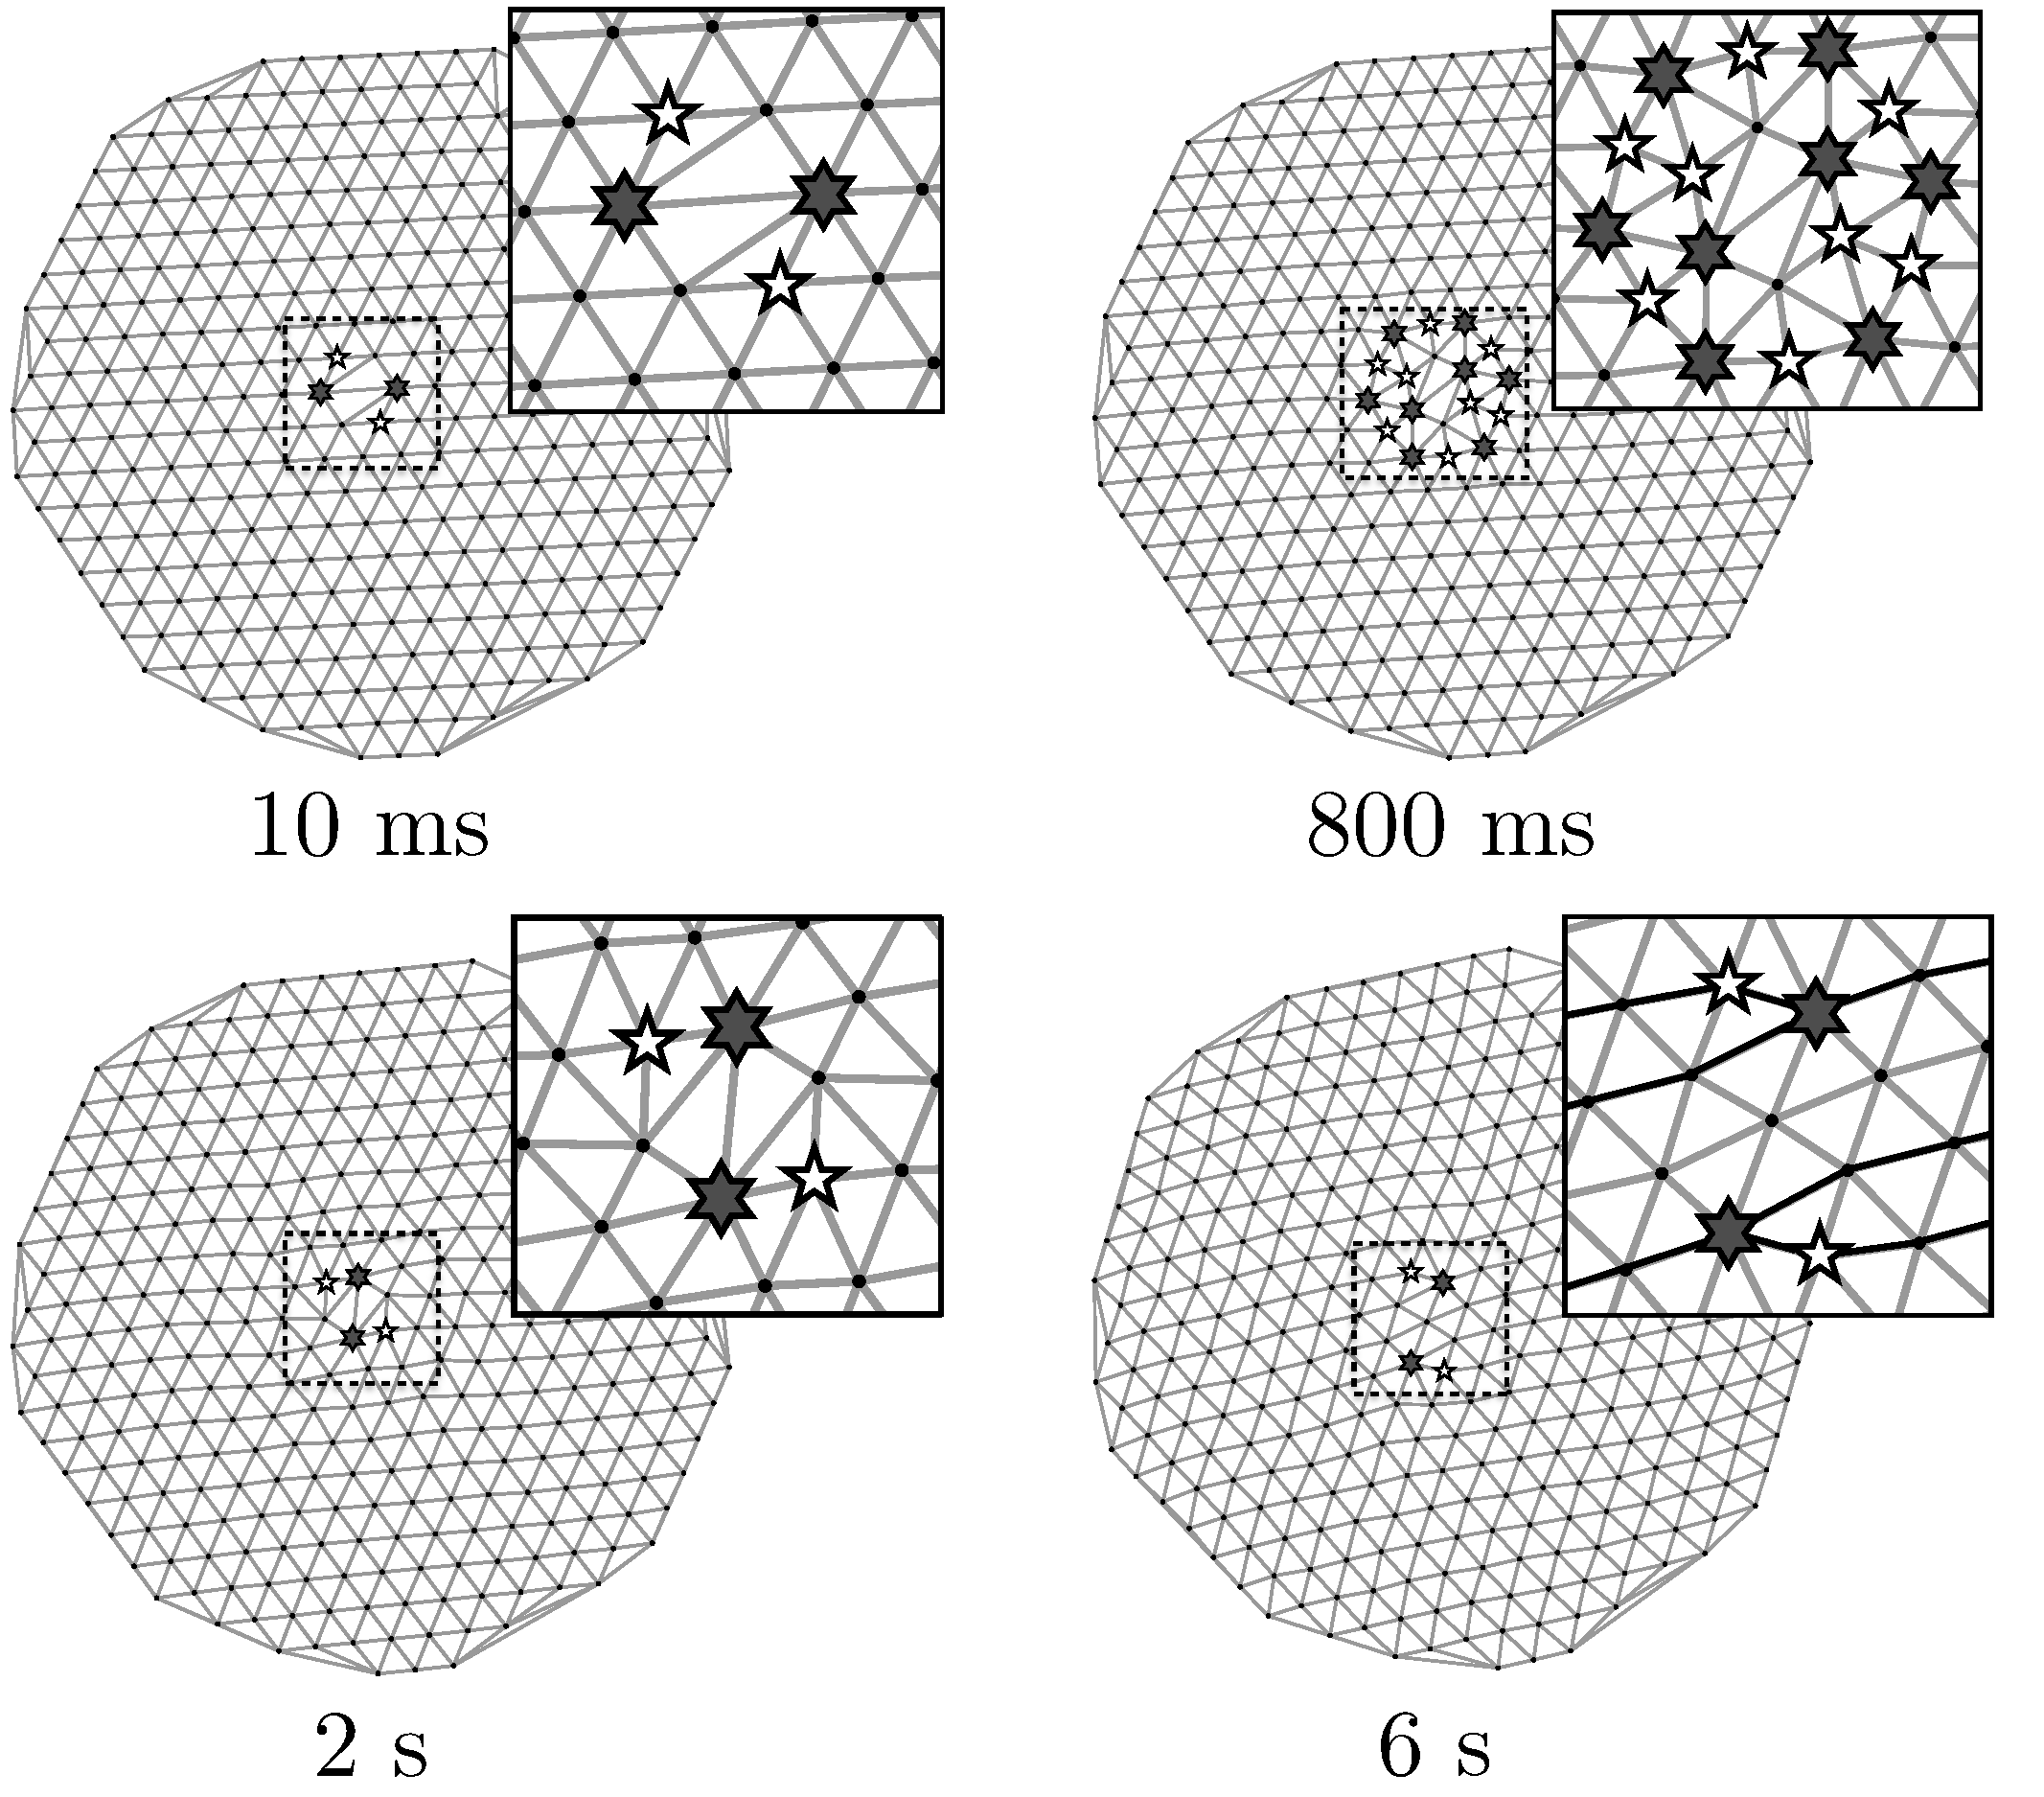
\includegraphics[width=0.55\textwidth]{ch5_kickit/fig6}
	\caption[Size of the resulting moir\'e super-structures as a function of the relative angle between the vortex and optical lattice.]{The dashed green line indicates the condensate radius. Inset: The different vectors in $\mathbf{k}$-space of the two lattices, with the optical lattice rotated by an angle $\theta_\Delta$. The $\mathbf{g}_{ll'} = |\mathbf{g}_l - \mathbf{g}_l'|$ vectors defining the dominant moir\'e wavelength are those for which the enclosed angle is smallest. }
	\label{fig:moire_lambda_1}
\end{figure}

    The appearance of the moir\'e vector in $\mathbf{k}$-space can be confirmed from the numerical simulations by looking at the compressible kinetic energy spectra which is given in Fig.~\ref{fig:dtheta_kspec}. Apart from the dominant peaks corresponding to the underlying triangular geometry of the Abrikosov lattice, which are independent of $\theta_\Delta$ (straight lines in Fig.~\ref{fig:dtheta_kspec}), a number of additional peaks appear. Their position is a function of the misalignment angle and the lowest wave-number that appears increases its value with increasing $\theta_\Delta$. This is consistent with the moir\'e model and the appearance of density structures of differing size. Furthermore, a symmetric repeat of this structure about the $\theta_\Delta=\pi/6$ point is also visible, which corresponds to the $\pi/3 - \theta_\Delta$ lattice vector component. The minimum wavelength observed agrees with the theoretically determined minimum value of $\lambda_M\approx 1.93\,a$ and all other values over the range of observed angles. Note that for the higher harmonics at larger wave-numbers similar behaviour exists and is also covered by the moir\'e model.
	\begin{figure}[tb]
        \centering
		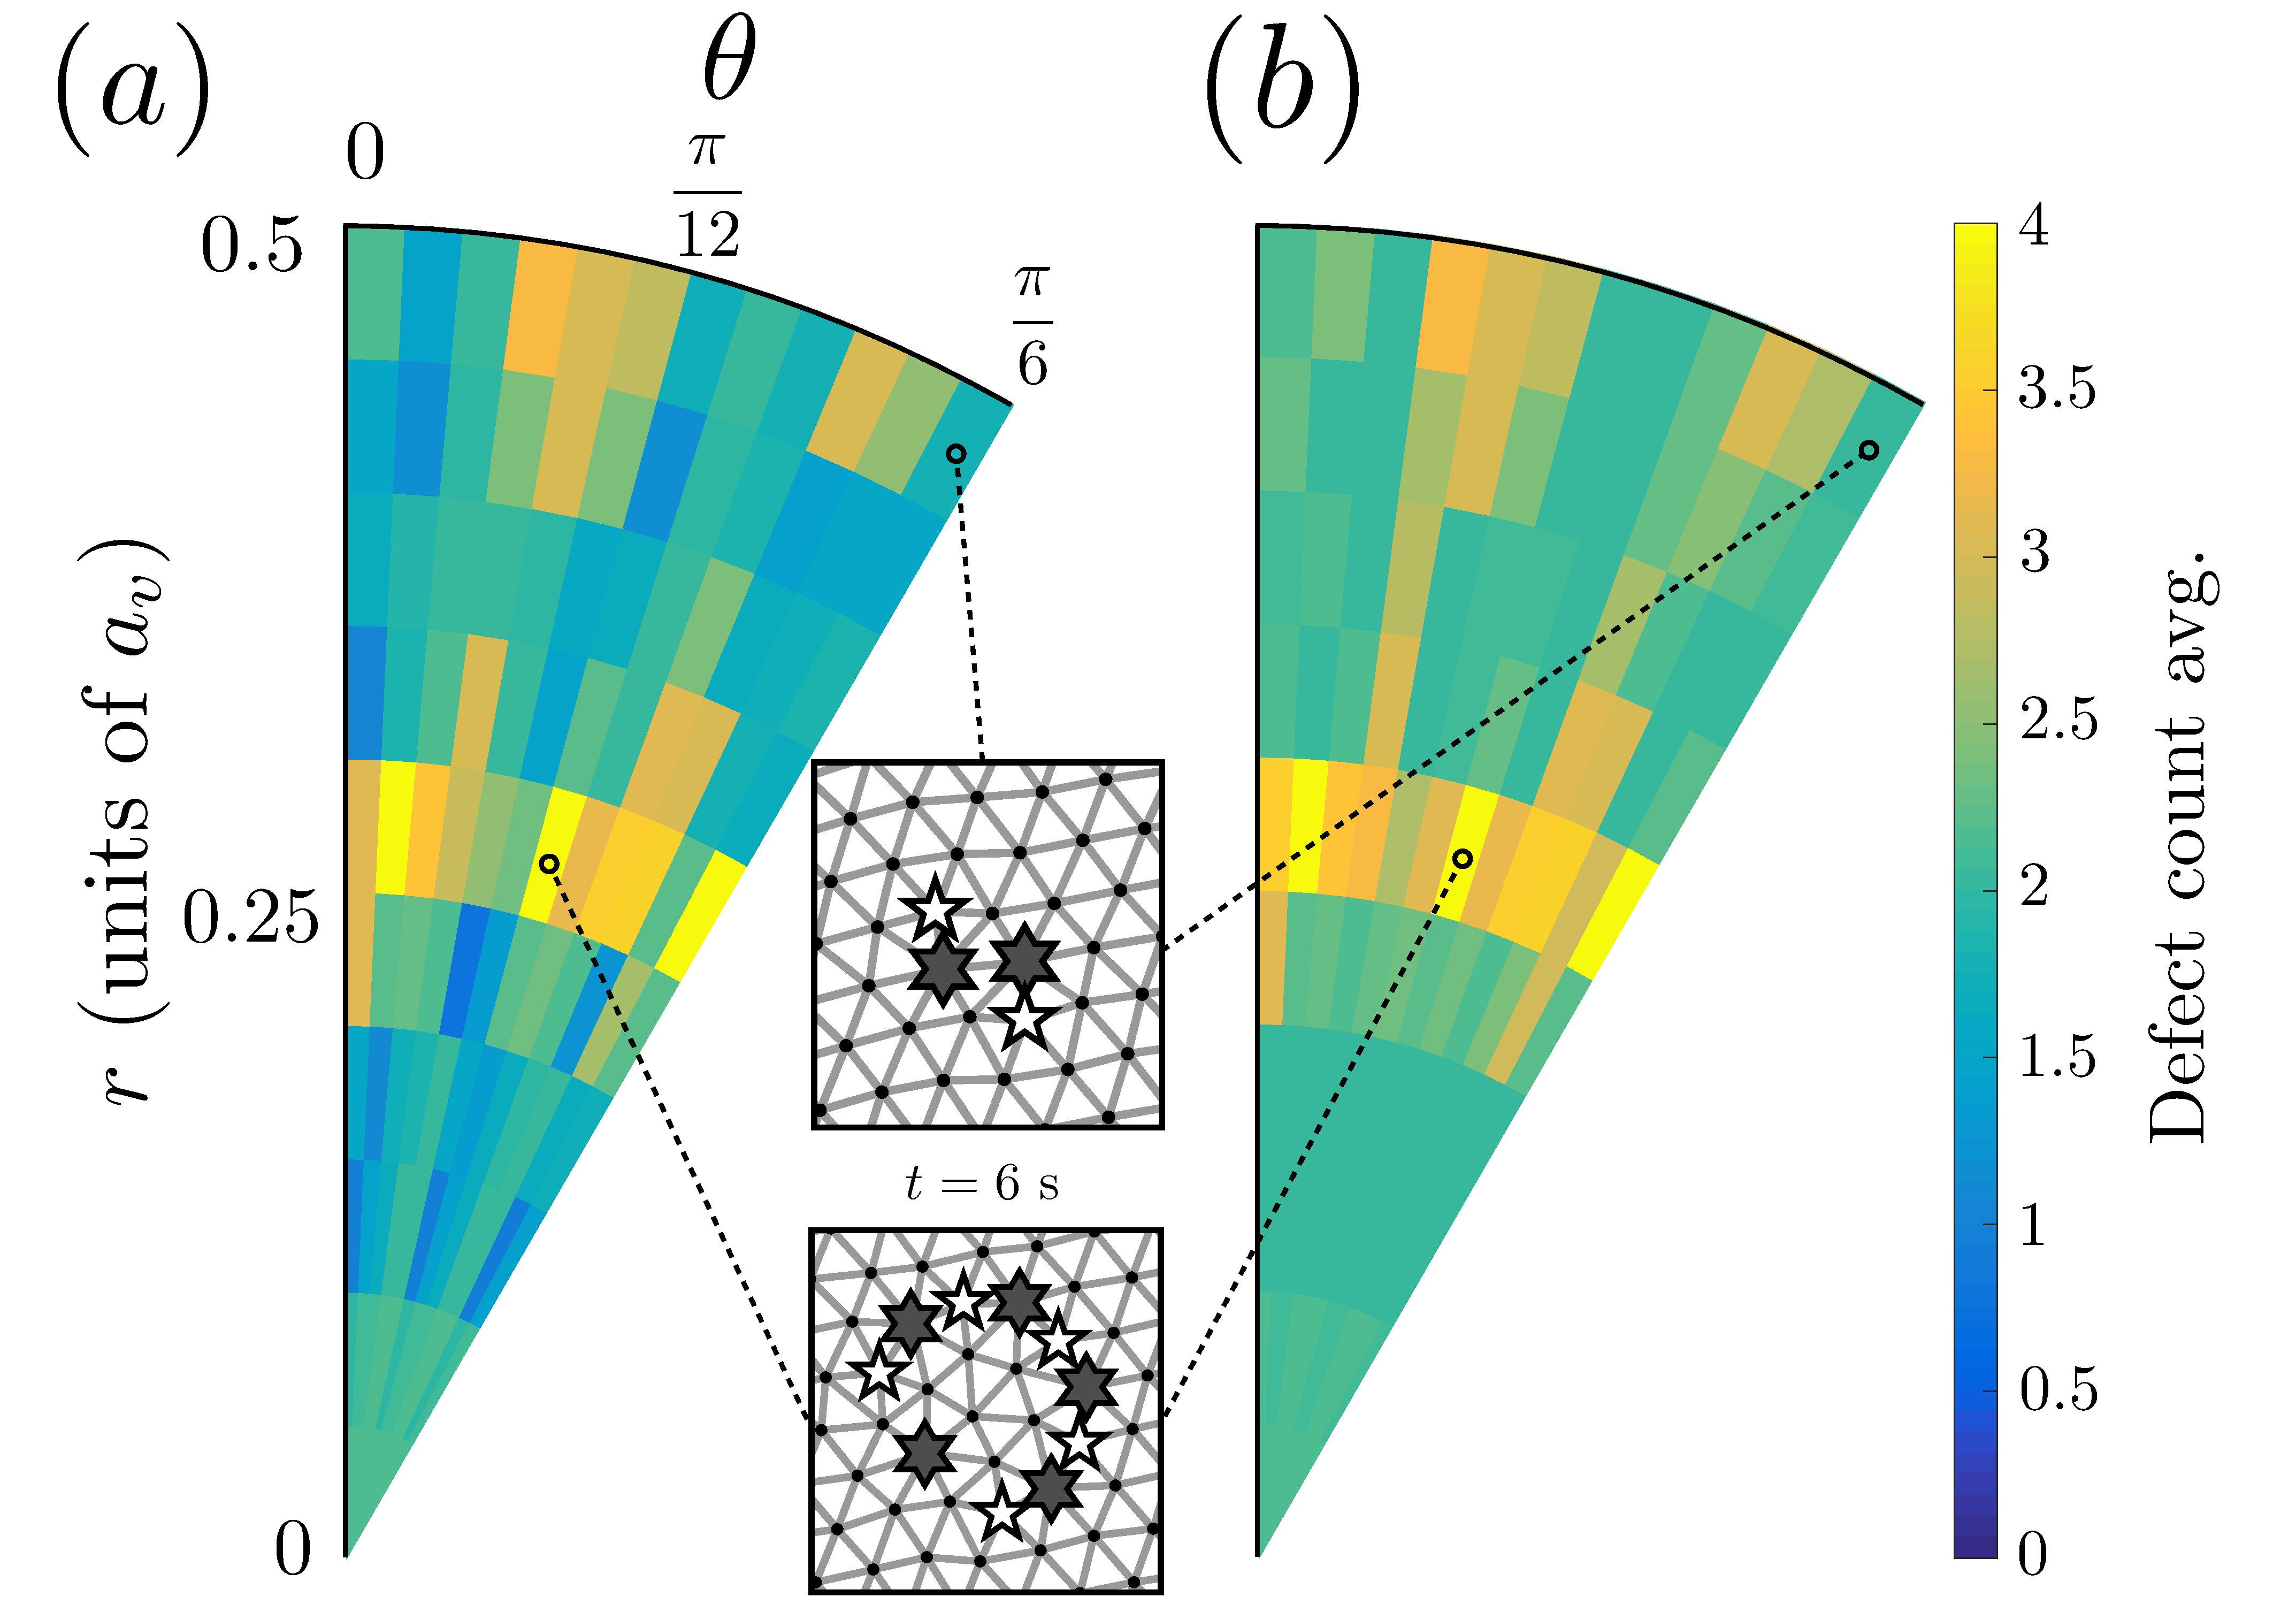
\includegraphics[width=0.55\textwidth]{ch5_kickit/fig7}
		\caption[Compressible kinetic energy spectrum as a function of $\theta_\Delta$.]{Compressible kinetic energy spectrum as a function of $\theta_\Delta$. All values are time-averaged over an interval $t=0$ s to $t=1$ s. The moir\'e peak corresponding to the lowest wave-number can be seen shifting to larger values for increasing angles and similar behavior is visible for the higher order components.}
		\label{fig:dtheta_kspec}
	\end{figure}
    \begin{figure}[tb]
        \centering
        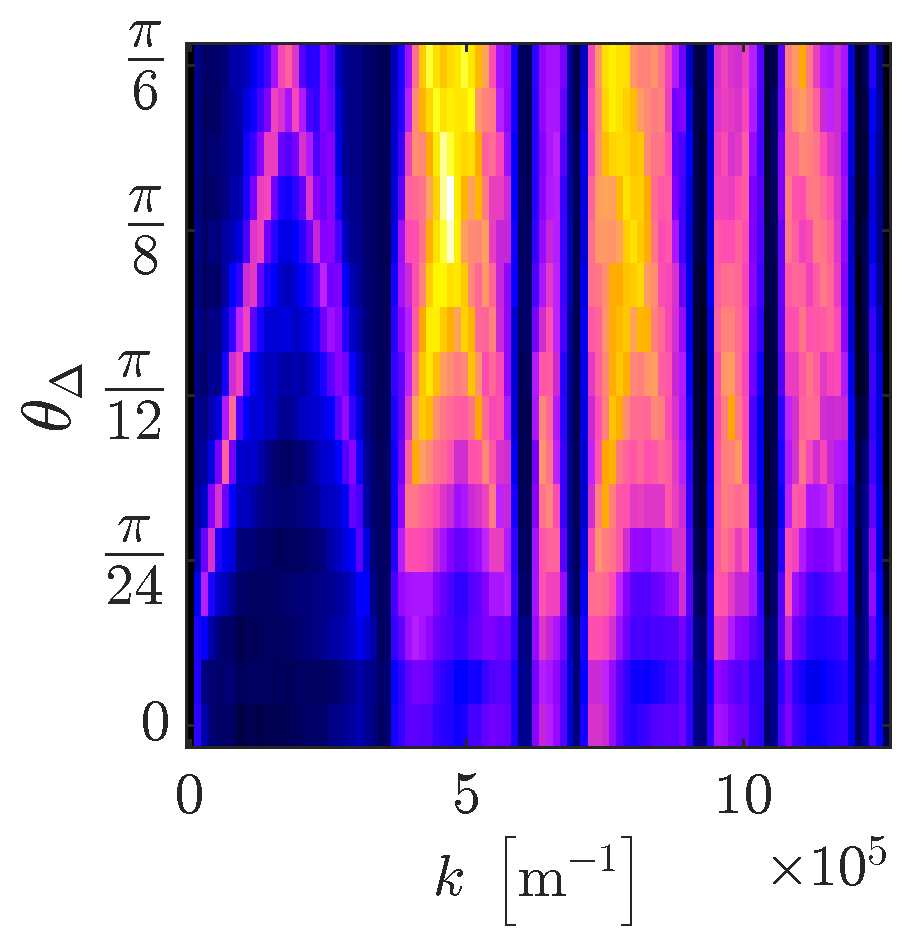
\includegraphics[width=0.55\textwidth]{ch5_kickit/theta_sweep_diff}
        \caption[Compressible kinetic energy spectrum with the background structure removed.]{Compressible kinetic energy spectrum with the static background structure removed. The effect of the moir\'e interference pattern for lower and higher modes is more easily visualised, compared with Fig. \ref{fig:dtheta_kspec}.}
        \label{fig:dtheta_kspec_backg}
    \end{figure}

    I will now briefly discuss what happens for stronger kicking, or when the two lattices are non-commensurate. In the above the strength of the kicking pulse was chosen such that its perturbation only leads to a phase imprinting \cite{Vtx:Dobrek_pra_1999,BEC:Denschlag_sci_2000}, with minimal change to the initial density. If one increases the kicking intensity the situation becomes quite different and one can see from Fig.~\ref{fig:kickp20k}(a) that higher order wave-numbers become more strongly excited. This, in turn, leads to modulations of the condensate density at shorter wavelength and an example is shown in Figs.~\ref{fig:kickp20k}(b)-(e), with the numerically calculated averaged spectra given in Fig.~\ref{fig:kick_compare_spec}. However, as for fully realistic experimental situations it is necessary to consider the heating of the condensates due to the disturbance once the kicking becomes stronger, I restrict this investigation to low intensity pulses.

\begin{figure}[tb]
    \centering
	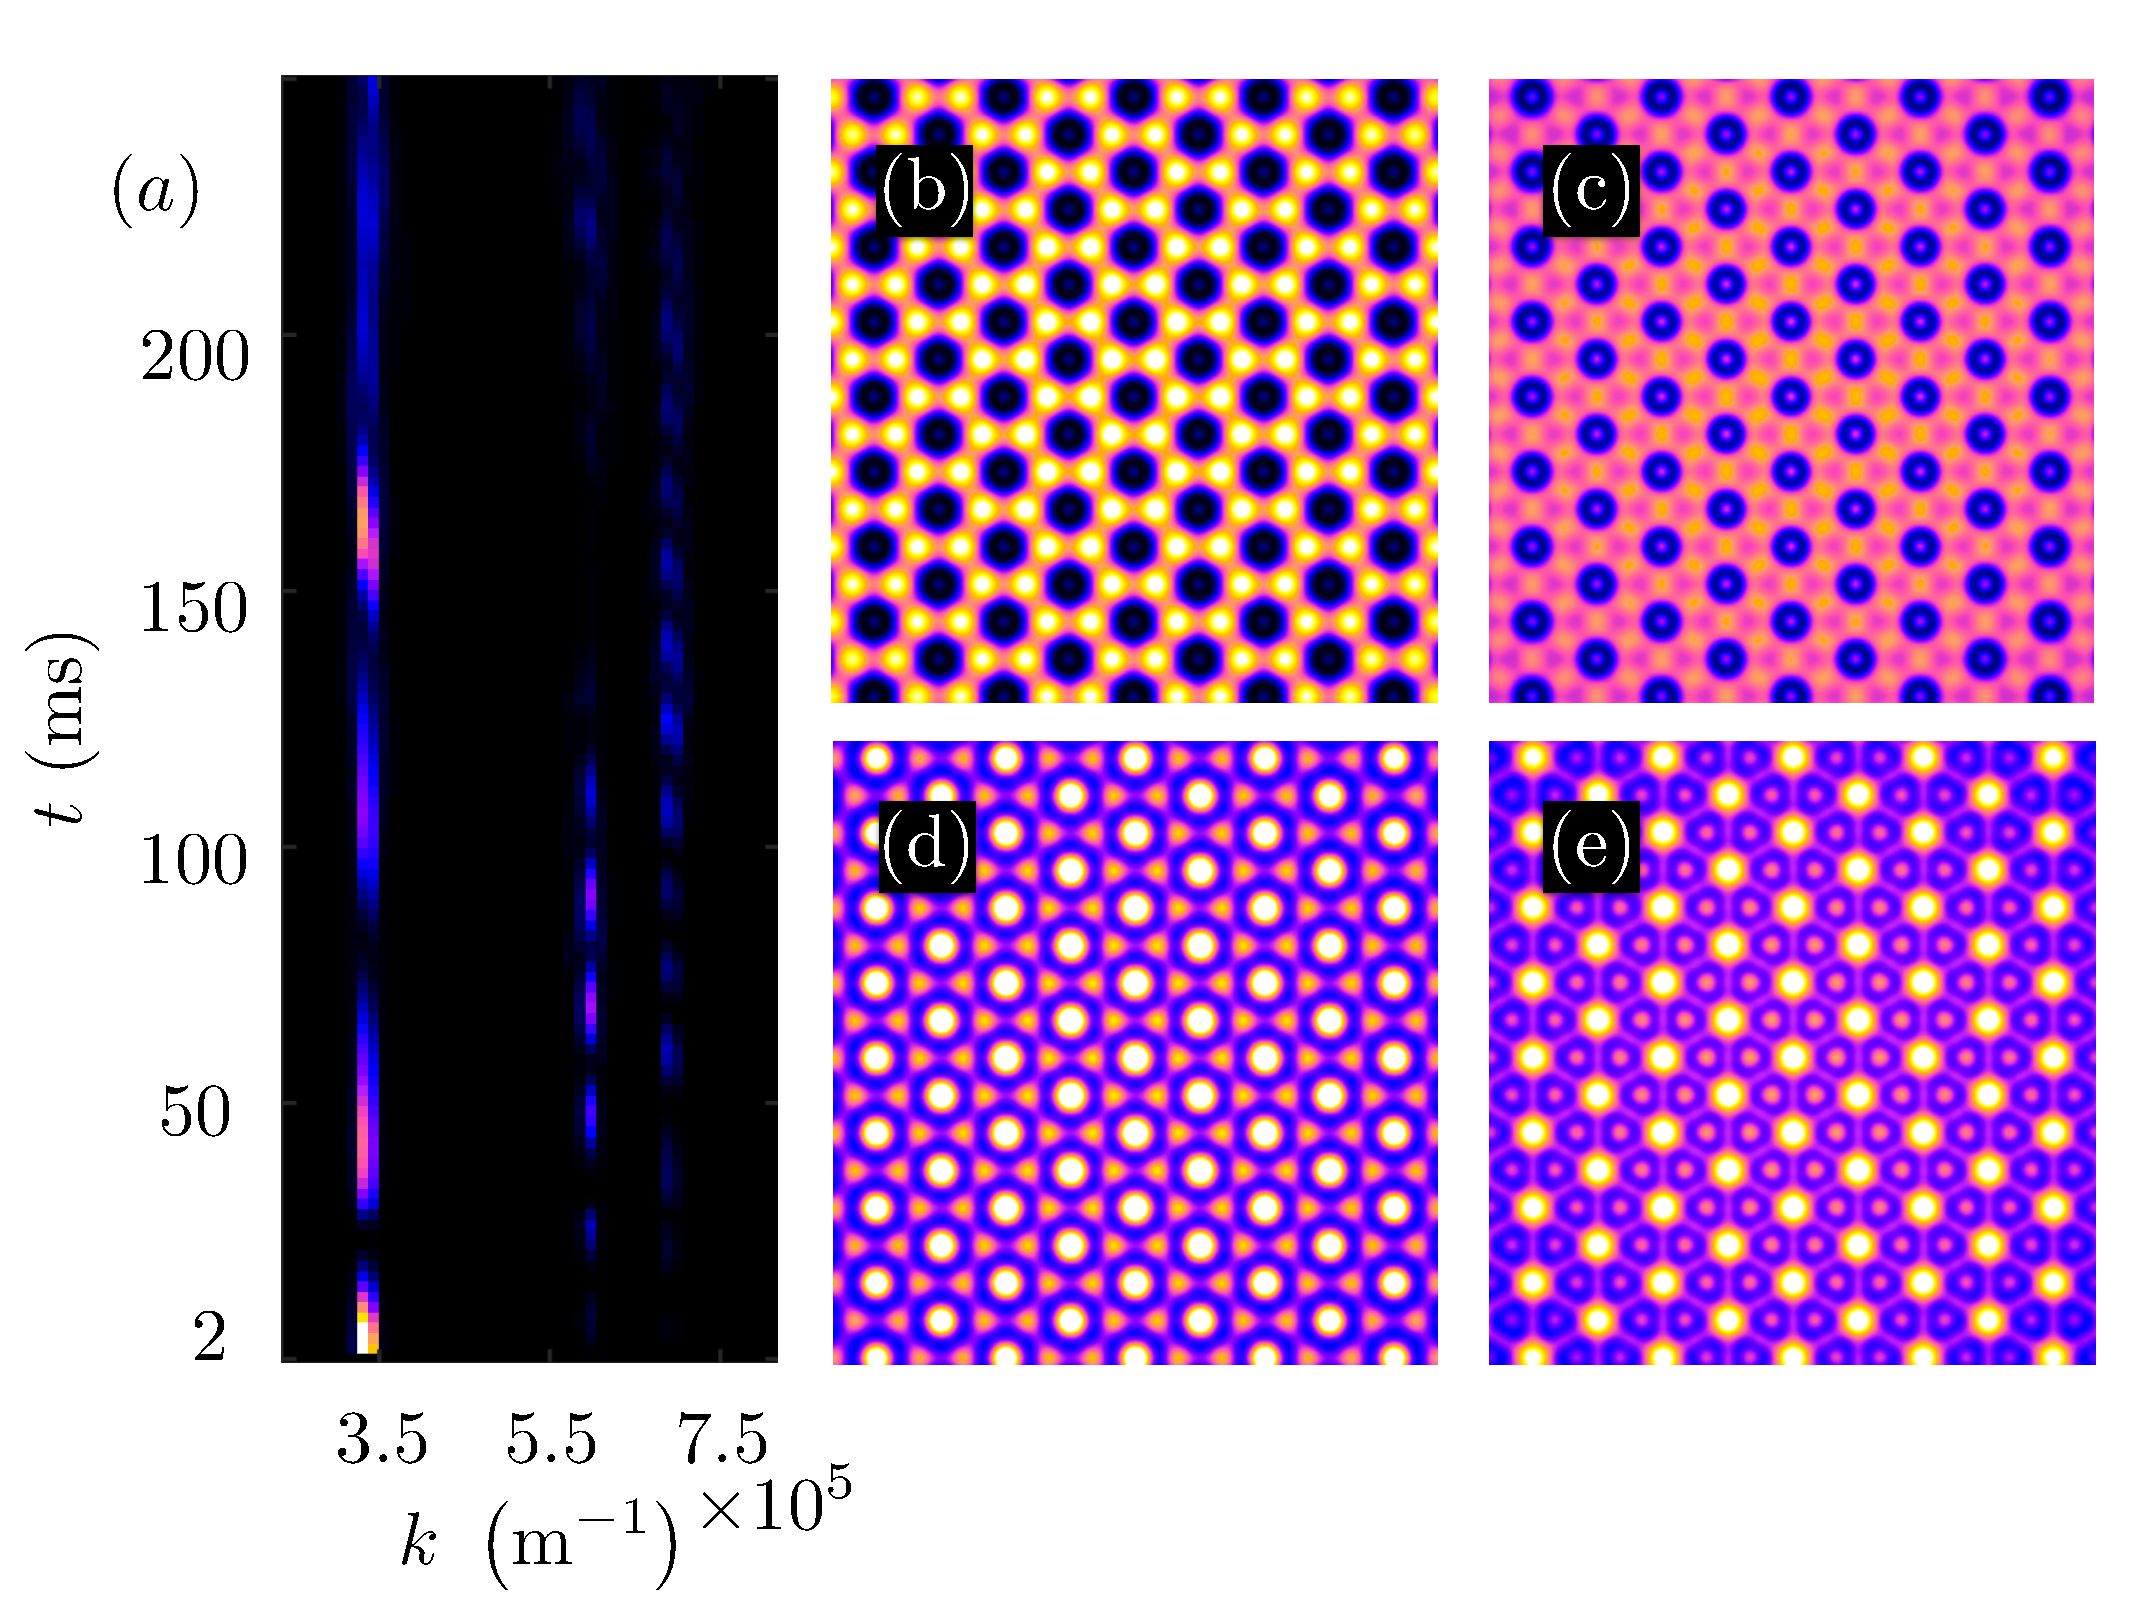
\includegraphics[width=0.55\textwidth]{ch5_kickit/fig8}
	\caption[Higher order modes induced by stronger kicking.]{(a) For a kicking strength of $V_0 = 5.4\times10^{-2}\mu$ for a non-rotating condensate higher order modes become non-negligible contributors to the compressible kinetic energy spectrum. This leads to a variety of different density structures, with some close-ups shown for (b) 24 ms, (c) 36 ms, (d) 56 ms, and (e) 88 ms. Note that the larger structures in these plots are given by the optical lattice constant, which sets the scale.}
	\label{fig:kickp20k}
\end{figure}
\begin{figure}[tb]
    \centering
    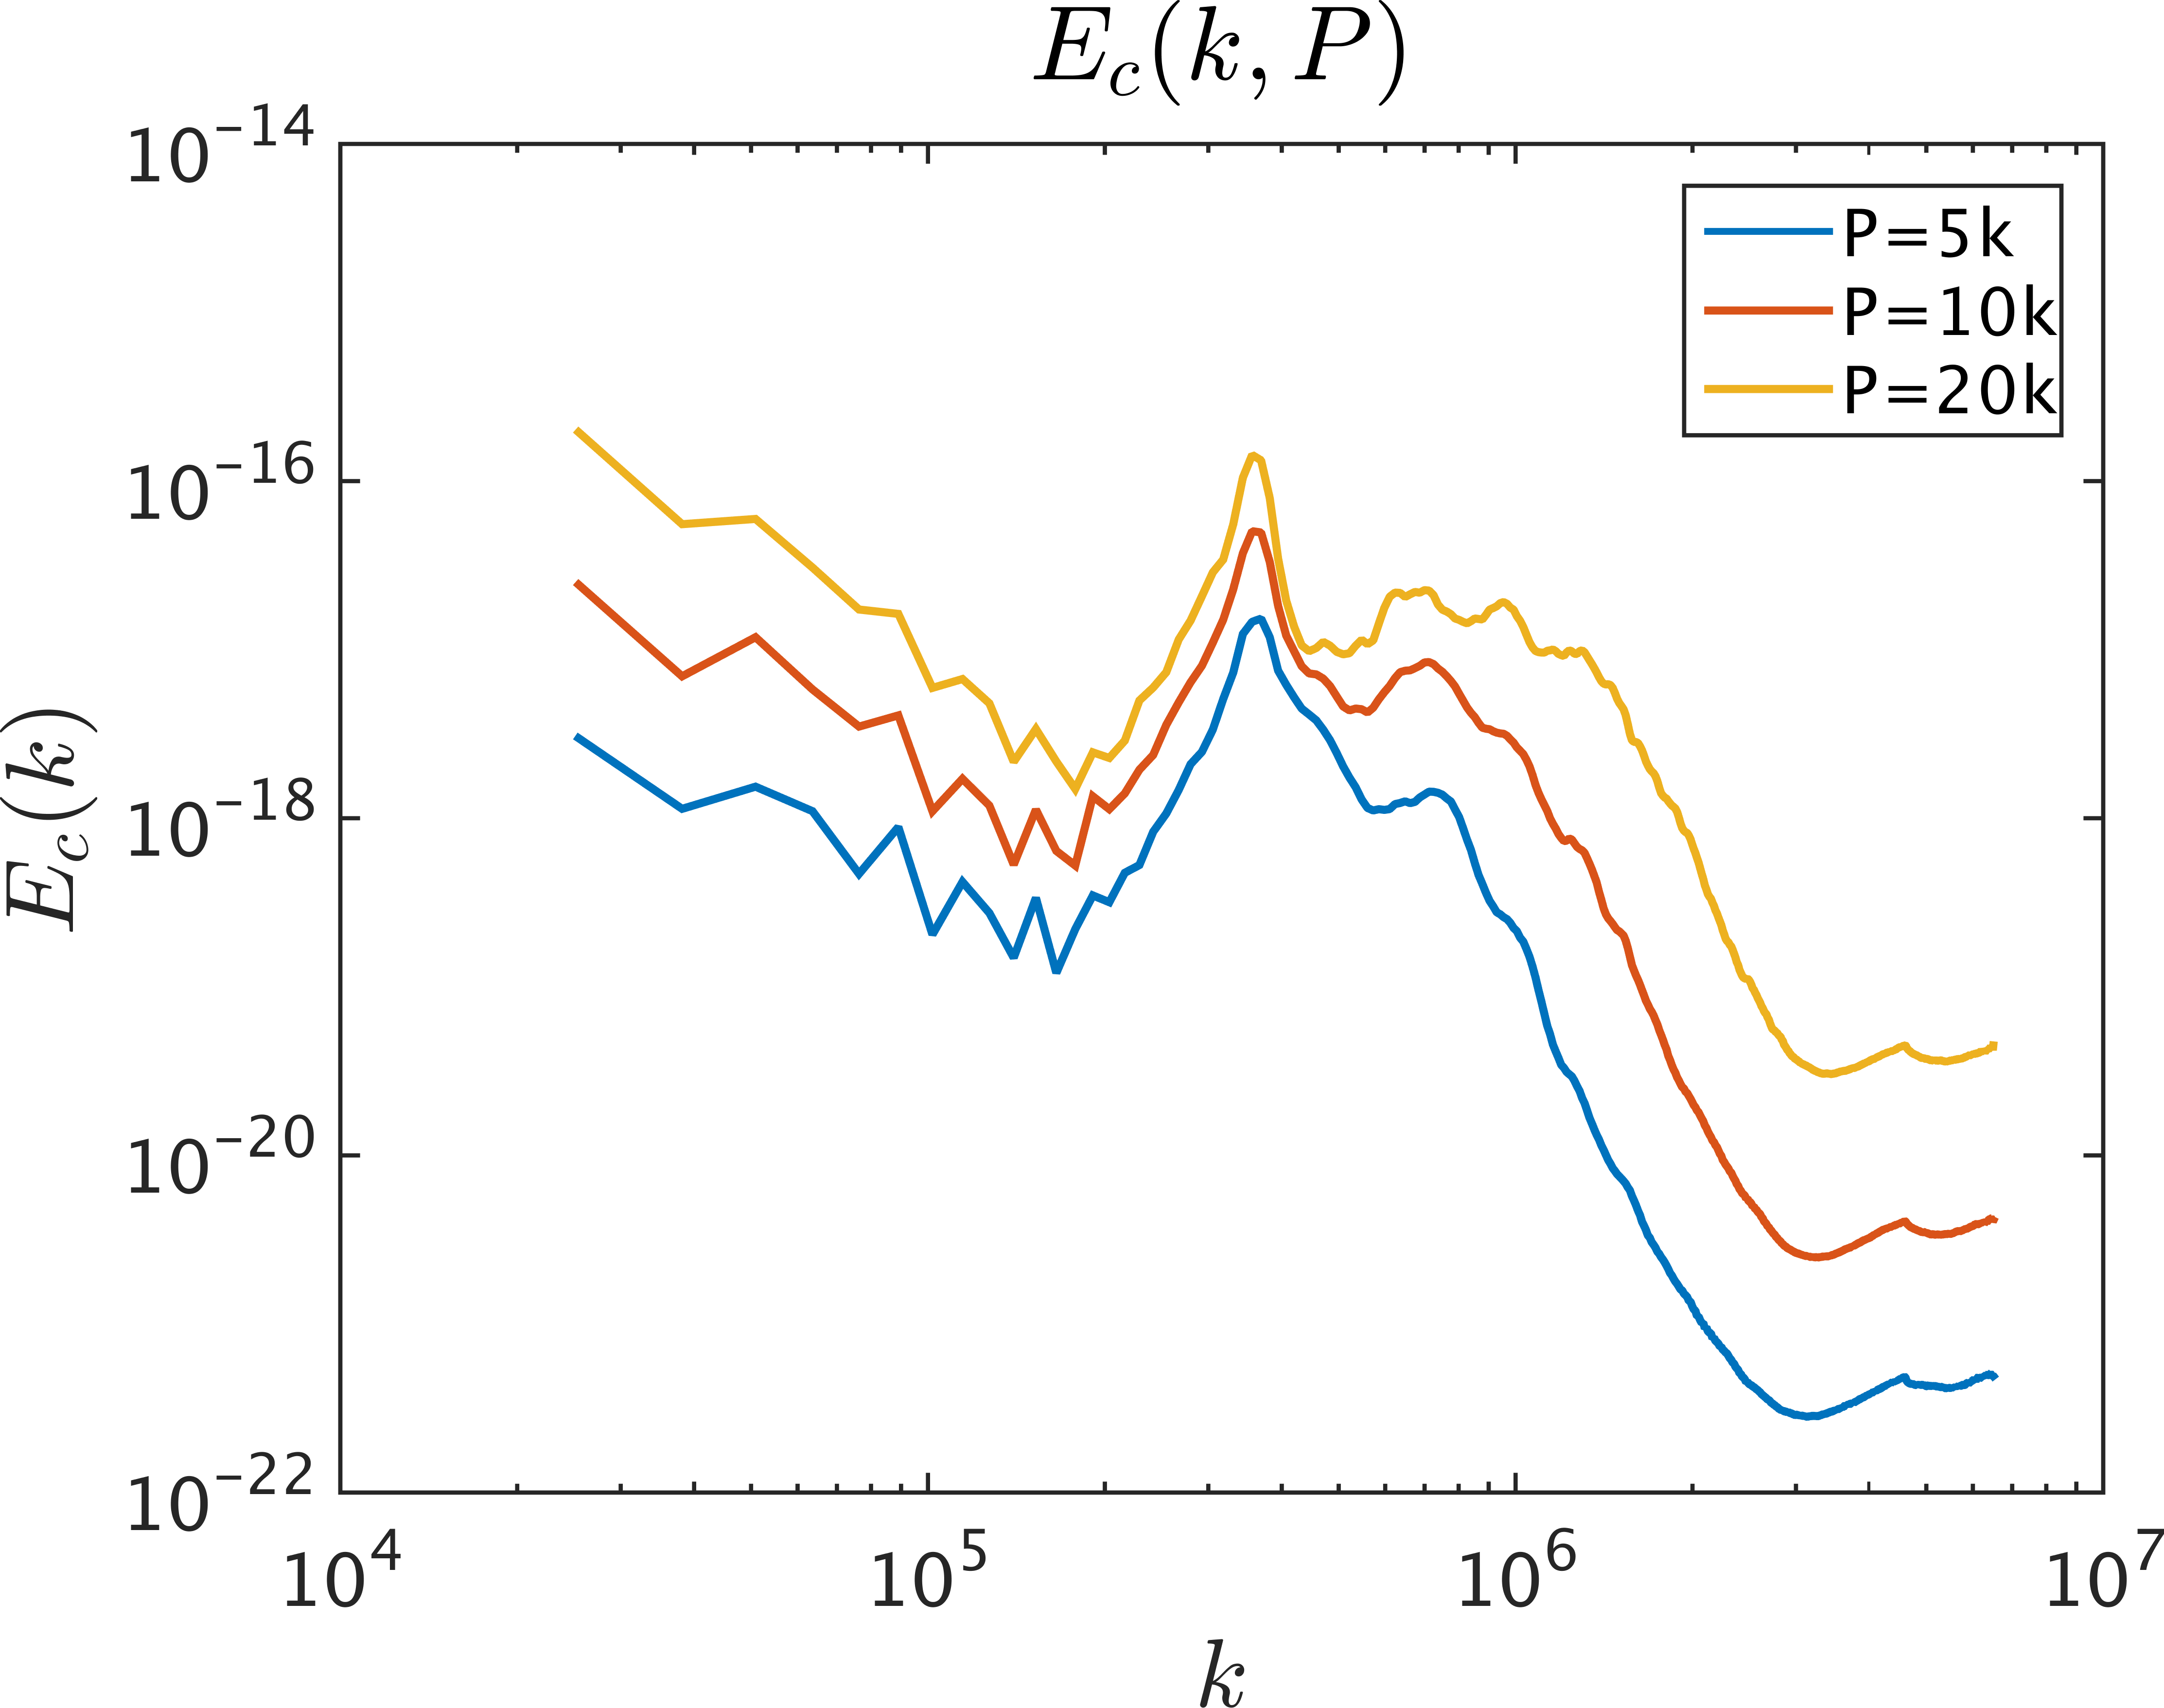
\includegraphics[width=0.49\textwidth]{ch5_kickit/EKc_novtx_tavg_p5k_10k_20k}
    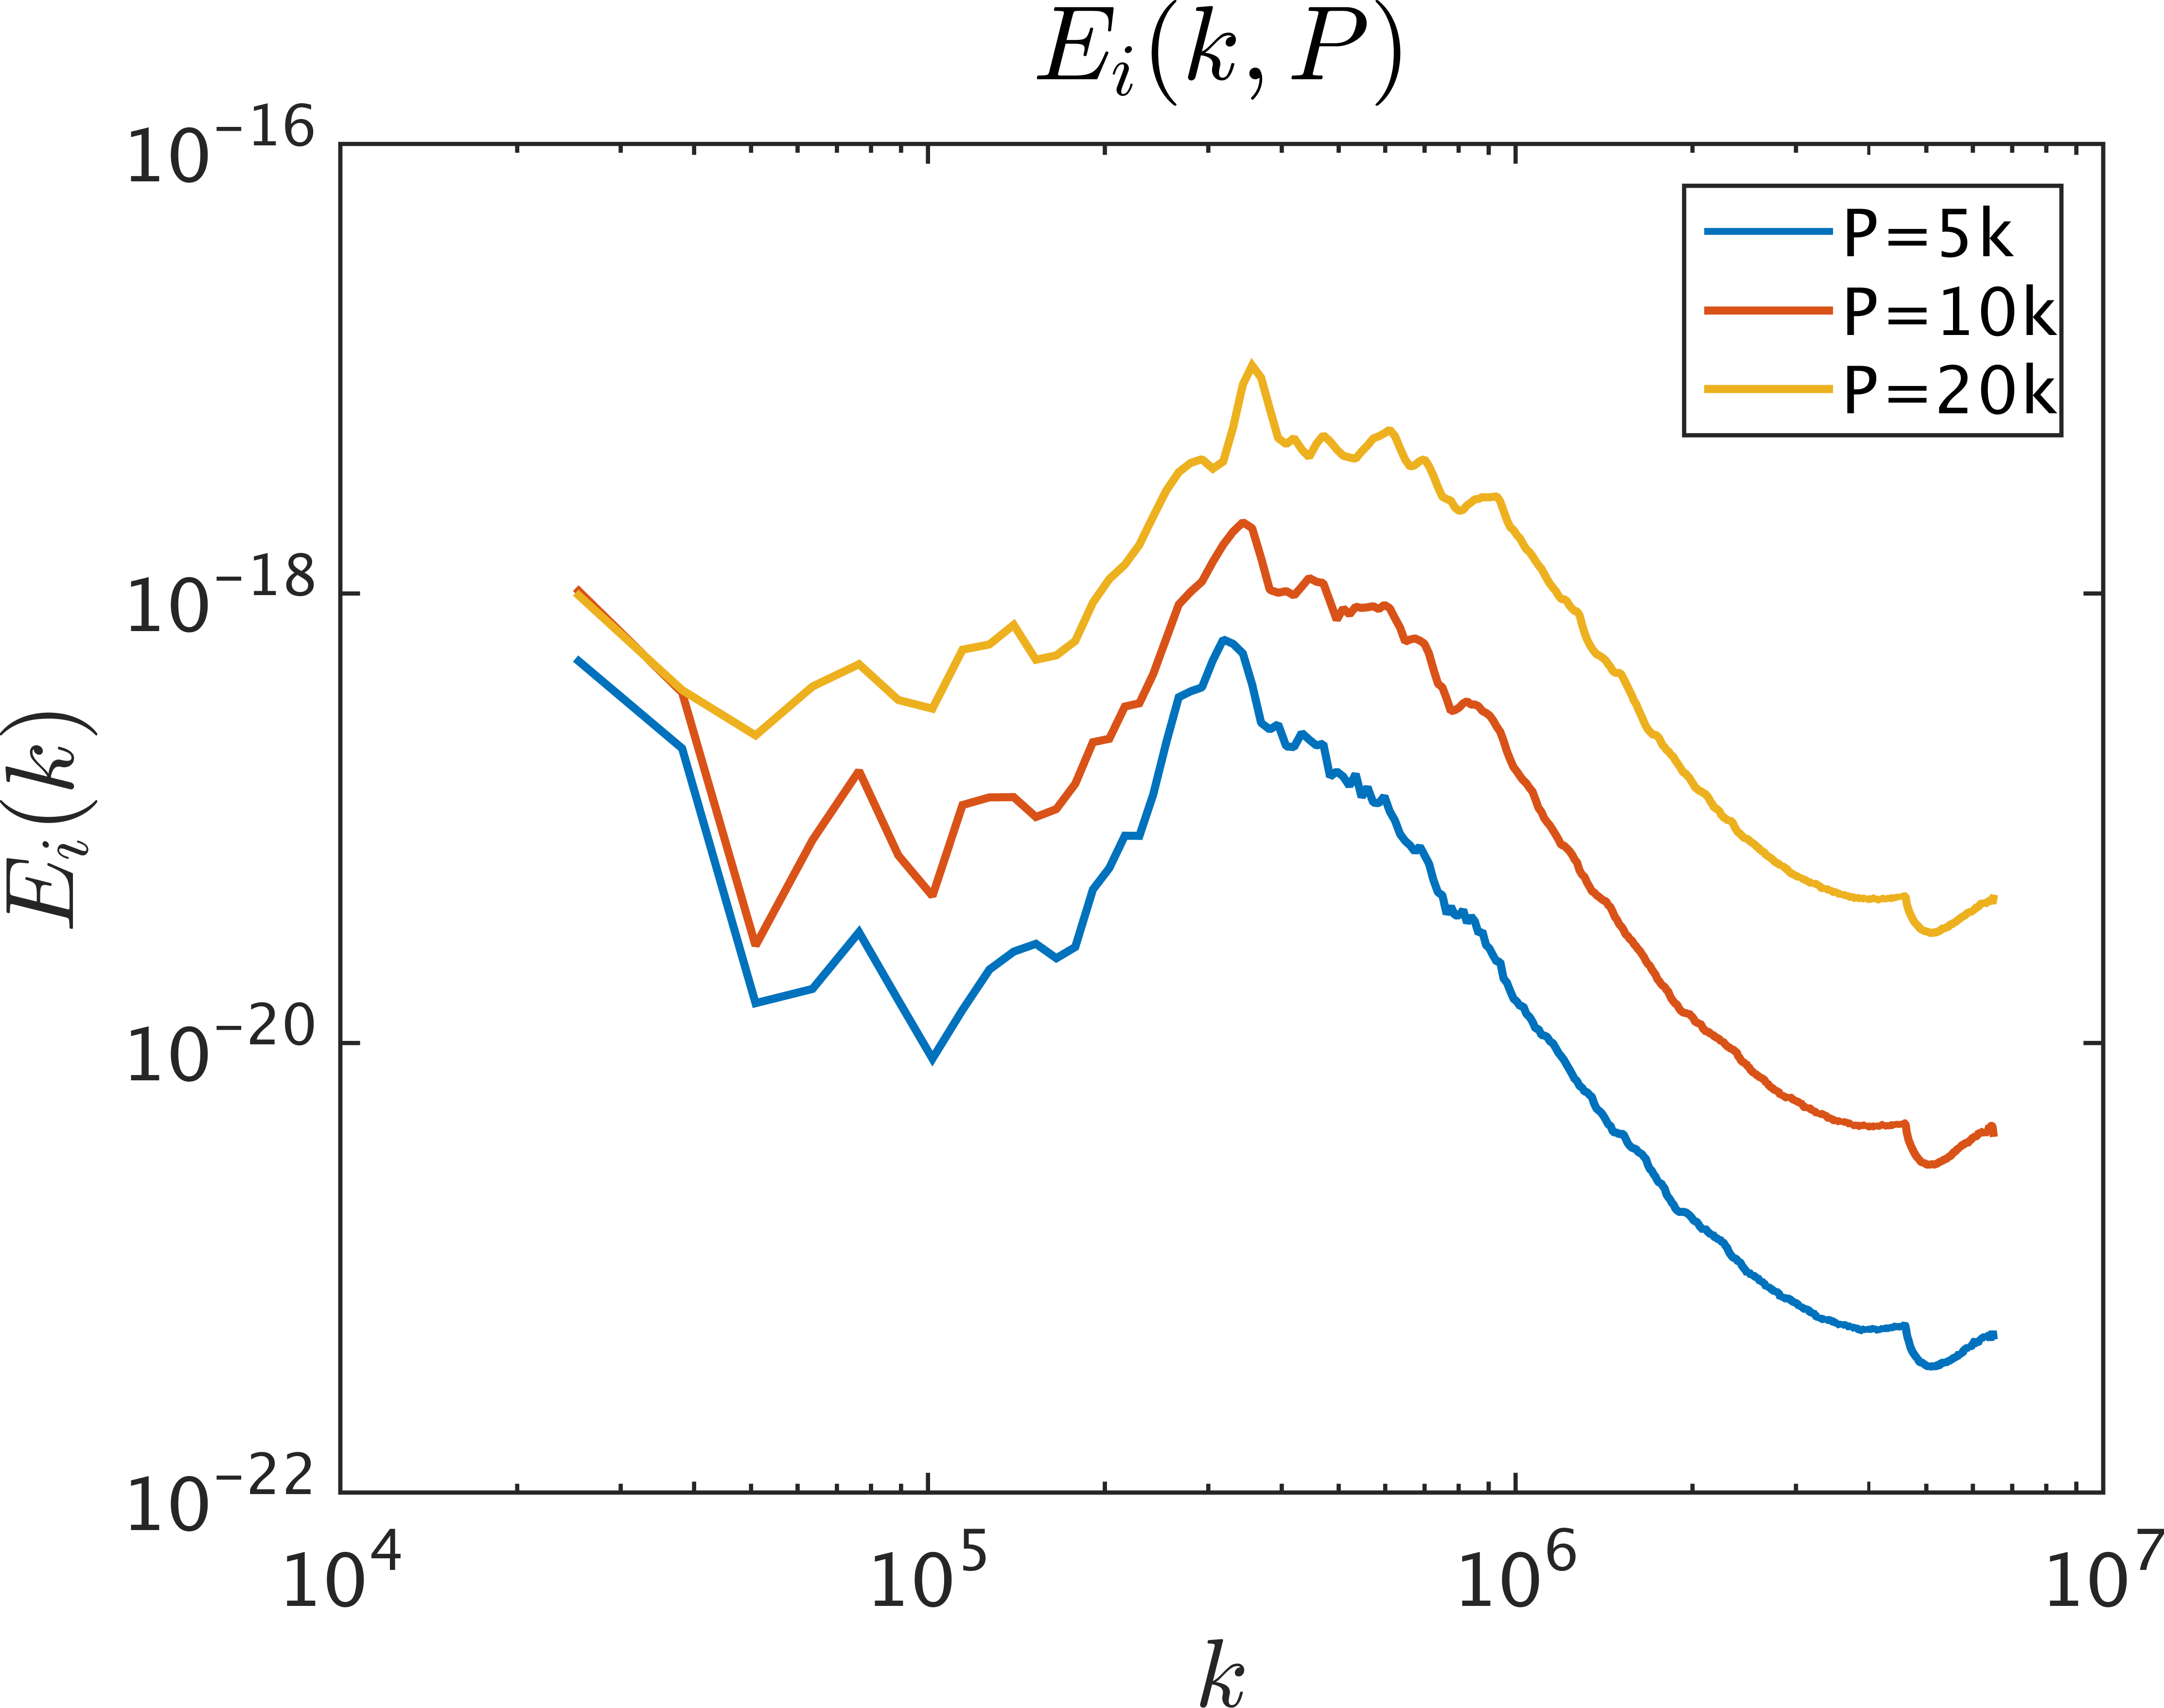
\includegraphics[width=0.49\textwidth]{ch5_kickit/EKi_novtx_tavg_p5k_10k_20k}
	\caption[Comparison of kinetic energy spectra for increased kicking strengths.]{Numerically invetigating the effect stronger kicking pulses have on the imparted kinetic energies show a clear increase in higher order modes being excited with an increase in optical lattice amplitude, for both compressible ($E_c$) and incompressible ($E_i$) cases.}\label{fig:kick_compare_spec}
\end{figure}

    A situation where the optical and the vortex lattice have different lattice constants can be imagined to appear naturally due to experimental uncertainties. Defining $a_o = a_v(1+\epsilon)$ the expression in eq.~\eqref{eq:InterferenceVectors} can be calculated to be
    \begin{equation}
    	\lambda_M = \frac{a_v(1+\epsilon)}{\sqrt{2(1+\epsilon)(1-\cos\theta) + \epsilon^2}}
    	\label{eqn:moire_size_eps}
    \end{equation}
    which reduces to eq.~\eqref{eqn:moire_size} for $\epsilon=0$. Evaluating this expression shows that the largest moir\'e wavelength changes slightly for small values of $\epsilon$, but it remains distinct enough from the underlying wave-vectors to stay visible in the evolution. This ensures that the system examined here is experimentally realistic.

\section{Conclusions}
\label{sec:ch5_conc}
While originally the intent of the proposed system was to investigate chaotic dynamics, it was instructive to investigate the interference pattern resulting from the kicking. As observed in the incompressible spectrum, kicking gave negligible effect to the vortex positions, with the lattice remaining well defined with near constant spacings, even in the long time limit. The optical lattice kicks solely modified the background density around the cores. One could observe that the vortex lattice remains incredibly stable and strongly resilient to perturbations and modulations in density. Given the stability of the lattice, it is expected that for a finite number of kicks, the lattice will remain unbroken. It is also expected that heating effects would play a role in destabilising the condensate, and to determine any such chaotic behaviour from this system, a non-negligible thermal cloud contribution would be necessary.

While not initially expected, this interference effect had some nice consequences. As a tool to test the periodidicity of a structure that is too small to resolve without time of flight, the moir\'e super-lattice structure may be useful for just that. Carrying out preliminary work in zig-zag and linear crystals in conjunction with A. Barahmi and Th. Busch, it was observed that without well defined periodic behaviour there is negligible observation of any peaks in the compressible energy spectrum. As such, there was negligible discernible moir\'e patterns in the density. It is expected that for such an effect to be useful highly periodic systems are required, with well defined wave-vectors. It remains an open question as to whether this can be used in a realistic experimental setting for such a purpose.
